\documentclass[11pt,a4paper]{article}

% ============================================================
% PAQUETES
% ============================================================
\usepackage[utf8]{inputenc}
\usepackage[T1]{fontenc}
\usepackage[spanish,es-nodecimaldot]{babel}
\usepackage{lmodern}
\usepackage{graphicx}
\usepackage{geometry}
\usepackage{array}
\usepackage{amsmath}
\usepackage{hyperref}

% ============================================================
% CONFIGURACIÓN DE PÁGINA
% ============================================================
\geometry{
    top=1.5cm,
    bottom=1.5cm,
    left=2.5cm,
    right=2.5cm
}

\setlength{\parindent}{0pt}
\setlength{\parskip}{0.5em}
\pagestyle{empty}

% Línea horizontal para secciones principales
\newcommand{\sectionline}{%
    \vspace{-0.6em}
    \noindent\rule{\textwidth}{0.5pt}
    \vspace{0.5em}
}

\begin{document}

% ============================================================
% PORTADA
% ============================================================

\begin{titlepage}

\begin{center}

{\normalsize\itshape
``Año de la Recuperación y Consolidación de la Economía Peruana''}

\vspace{0.35cm}

\resizebox{0.86\textwidth}{!}{%
    \textbf{UNIVERSIDAD NACIONAL DE INGENIERÍA}%
}

\vspace{0.30cm}

{\Large\bfseries
FACULTAD DE CIENCIAS}

\vspace{0.35cm}

{\Large\bfseries
FÍSICA II}

\vspace{0.30cm}


\includegraphics[width=4.5cm]{../figuras/imagen_uni_escudo.png}

\vspace{0.25cm}

{\Large\bfseries ESCUELA DE FÍSICA}\\[0.12cm]

{\Large\bfseries LABORATORIO 1}

\vspace{0.35cm}

{\Large\bfseries\itshape
DETERMINACIÓN DEL MOMENTO DE INERCIA\\[0.12cm]
DE UN DISCO Y DE UN ANILLO}

\end{center}

% ============================================================
% SECCIÓN Y FECHA
% ============================================================

\vspace{1.15cm}

\noindent
\begin{tabular*}{\textwidth}
{@{\extracolsep{\fill}}ll}

{\large\textbf{SECCIÓN:} B}
&
{\large\textbf{DÍA Y HORA:} 01/09/2026 -- 1:00 p.\,m.}

\end{tabular*}

% ============================================================
% INTEGRANTES
% ============================================================

\vspace{0.90cm}

\renewcommand{\arraystretch}{1.45}

\begin{center}

{\large
\begin{tabular}{|p{9.7cm}|p{3.4cm}|}
\hline

\textbf{APELLIDOS Y NOMBRES}
&
\textbf{CÓDIGO}
\\
\hline

Macuri Torres, Alessandro Omar
&
20250652J
\\
\hline

Moreno Cabanillas, Alexandra Romina
&
20251764F
\\
\hline

\end{tabular}
}

\end{center}

% ============================================================
% DOCENTES
% ============================================================

\vspace{0.85cm}

{\large\textbf{NOMBRE DE LOS DOCENTES:}}

\vspace{0.35cm}

{\large
\hspace{0.6cm}
-- CORTEZ REYES, Gregorio Custodio

\vspace{0.20cm}

\hspace{0.6cm}
-- SILVA VÁSQUEZ, Humberto Martín
}

% ============================================================
% FECHA DE ENTREGA
% ============================================================

\vspace{0.95cm}

{\large
\textbf{FECHA DE ENTREGA DEL INFORME:}
\hspace{0.40cm}
15/09/2026
}

% ============================================================
% PERIODO ACADÉMICO
% ============================================================

\vspace{1.15cm}

\begin{center}
{\huge\bfseries 2026--II}
\end{center}

\end{titlepage}

% ============================================================
% ÍNDICE
% ============================================================

\newpage
\tableofcontents
\newpage


% ============================================================
% INTRODUCCIÓN
% ============================================================

\newpage

\section*{INTRODUCCIÓN}
\addcontentsline{toc}{section}{INTRODUCCIÓN}
\sectionline

La participación y las contribuciones individuales de cada integrante en el
desarrollo de la experiencia y la elaboración del presente informe se detallan
en la sección de anexos.

El estudio de la dinámica rotacional constituye uno de los pilares de la
mecánica clásica. Desde los primeros estudios sistemáticos de Galileo Galilei
sobre el movimiento de los cuerpos hasta la formulación de las leyes de la
mecánica por Isaac Newton, la descripción de la rotación ha desempeñado un
papel fundamental en la comprensión del comportamiento de los cuerpos rígidos.
En este contexto, el momento de inercia representa una magnitud esencial, pues
cuantifica la resistencia de un cuerpo a modificar su estado de rotación
alrededor de un eje determinado y desempeña, en la dinámica rotacional, un
papel análogo al de la masa en el movimiento traslacional.

El momento de inercia no depende únicamente de la masa total de un cuerpo,
sino también de la distribución de dicha masa respecto del eje de rotación.
En consecuencia, dos cuerpos de masas semejantes pueden presentar respuestas
dinámicas diferentes ante la aplicación de un mismo torque si sus
distribuciones de masa son distintas. El disco y el anillo constituyen ejemplos
particularmente apropiados para estudiar este fenómeno, ya que presentan
distribuciones de masa diferentes y sus momentos de inercia pueden determinarse
teóricamente a partir de sus masas y dimensiones geométricas.

En el presente laboratorio se determina experimentalmente el momento de
inercia de un disco y de un anillo mediante un sistema rotacional accionado
por una masa suspendida. Durante el descenso de esta masa, la tensión del hilo
ejerce un torque sobre el sistema y produce una aceleración angular. La
aceleración lineal de la masa suspendida se obtiene a partir de la pendiente
del ajuste de la gráfica de velocidad en función del tiempo y, mediante las
relaciones entre la dinámica traslacional y rotacional, se emplea para
determinar el momento de inercia experimental del sistema.

Finalmente, los valores experimentales del momento de inercia se comparan con
los obtenidos teóricamente a partir de las masas y dimensiones geométricas del
disco y del anillo. En el análisis se consideran las incertidumbres asociadas
a las magnitudes medidas y su correspondiente propagación, con el propósito
de evaluar cuantitativamente la concordancia entre las predicciones del modelo
teórico y los resultados experimentales, así como identificar las principales
fuentes de discrepancia.


% ============================================================
% RESUMEN
% ============================================================

\newpage
\section*{RESUMEN}
\addcontentsline{toc}{section}{RESUMEN}
\sectionline

En la presente experiencia se determinó experimentalmente el momento de
inercia de un sistema disco--anillo mediante el análisis de su dinámica
rotacional. La aceleración lineal de la masa suspendida se obtuvo a partir
de un ajuste lineal de 37 datos de velocidad en función del tiempo,
realizado mediante Python, obteniéndose
\(a=(0.00494258\pm0.00003125)\,\mathrm{m/s^2}\), con un coeficiente de
determinación \(R^2=0.998603\).

A partir de la aceleración y de los parámetros medidos del sistema se
determinó un momento de inercia experimental
\(I_{\mathrm{exp}}=(0.01716663\pm0.00017040)\,\mathrm{kg\,m^2}\).
Por otra parte, mediante las masas y dimensiones geométricas del disco y
del anillo se obtuvo un valor teórico total
\(I_{\mathrm{teo}}=(0.01452303\pm0.00008334)\,\mathrm{kg\,m^2}\).
La comparación entre ambos resultados produjo una discrepancia de
\(18.20\%\), superior a la explicable únicamente por las incertidumbres
propagadas. Esta diferencia se atribuye principalmente a efectos
sistemáticos no considerados en el modelo ideal, tales como la fricción
en el sistema, el momento de inercia de la polea y posibles variaciones
del radio efectivo de enrollamiento del hilo.

\newpage

\section*{OBJETIVOS}
\addcontentsline{toc}{section}{OBJETIVOS}
\sectionline

\subsection*{Objetivo general}

Determinar experimentalmente el momento de inercia de un disco y de un
anillo mediante el análisis de su dinámica rotacional, y comparar los
resultados obtenidos con los valores teóricos calculados a partir de sus
masas y dimensiones geométricas.

\subsection*{Objetivos específicos}

\begin{itemize}

    \item Determinar la aceleración lineal del sistema disco--anillo a
    partir de la pendiente obtenida mediante el ajuste de los datos de
    velocidad en función del tiempo.

    \item Calcular el momento de inercia experimental del sistema
    disco--anillo mediante la aplicación de la segunda ley de Newton y
    las ecuaciones de la dinámica rotacional.

    \item Calcular los momentos de inercia teóricos del disco y del
    anillo a partir de sus masas y dimensiones geométricas.

    \item Estimar las incertidumbres asociadas a las magnitudes
    determinadas mediante la correspondiente propagación de
    incertidumbres.

    \item Comparar cuantitativamente el momento de inercia experimental
    del sistema disco--anillo con su valor teórico, evaluando la
    discrepancia e identificando las principales fuentes de error
    experimental.

\end{itemize}


% ============================================================
% FUNDAMENTOS TEÓRICOS
% ============================================================

\newpage

\section*{FUNDAMENTOS TEÓRICOS}
\addcontentsline{toc}{section}{3. FUNDAMENTOS TEÓRICOS}
\sectionline


% ------------------------------------------------------------
% 3.1 DINÁMICA ROTACIONAL Y MOMENTO DE INERCIA
% ------------------------------------------------------------

\subsection*{3.1. Dinámica rotacional y momento de inercia}

La dinámica rotacional estudia el movimiento de los cuerpos alrededor de
un eje y su respuesta ante la acción de torques. Una de las magnitudes
fundamentales para describir este comportamiento es el \textbf{momento de
inercia}, el cual cuantifica la resistencia de un cuerpo a experimentar
cambios en su movimiento rotacional y depende tanto de su masa como de la
distribución de esta respecto del eje de rotación.

De acuerdo con Medina Guzmán (2010), el momento de inercia de un cuerpo
rígido respecto de un eje se determina considerando la distribución de sus
elementos de masa y sus respectivas distancias al eje de rotación. De forma
análoga, Serway y Jewett (2009) señalan que esta magnitud depende de la masa
del cuerpo, de su distribución y del eje alrededor del cual se realiza la
rotación.

Para un cuerpo con distribución continua de masa, el momento de inercia se
define mediante

\[
I=\int r^2\,dm,
\]

donde \(r\) representa la distancia perpendicular entre el elemento
diferencial de masa \(dm\) y el eje de rotación. Esta definición constituye
el punto de partida para obtener los momentos de inercia teóricos del disco
y del anillo.


% ------------------------------------------------------------
% 3.2 MOMENTO DE INERCIA DEL DISCO Y DEL ANILLO
% ------------------------------------------------------------

\subsection*{3.2. Momento de inercia de un disco y de un anillo}

El momento de inercia de un cuerpo rígido depende de su geometría y de la
distribución de su masa respecto del eje considerado. En la presente
experiencia se estudian un disco y un anillo homogéneos, ambos rotando
alrededor de un eje perpendicular a su plano y que atraviesa su centro
geométrico.

Según Halliday, Resnick y Walker (2009), el cálculo del momento de inercia
de un cuerpo rígido puede realizarse dividiendo el cuerpo en elementos
diferenciales de masa y sumando, mediante integración, la contribución de
cada elemento respecto del eje de rotación. Este procedimiento permite
obtener las expresiones particulares correspondientes a diferentes
distribuciones geométricas de masa.


% ------------------------------------------------------------
% 3.2.1 DISCO
% ------------------------------------------------------------

\begin{list}{}{\leftmargin=1.2cm\rightmargin=0cm}
\item[]

\textbf{3.2.1. Momento de inercia de un disco}

\vspace{0.3em}

Considérese un disco homogéneo de masa \(M\) y radio \(R\). Debido a que su
masa se encuentra distribuida uniformemente sobre su superficie, su densidad
superficial de masa es

\[
\sigma=\frac{M}{\pi R^2}.
\]

Para determinar su momento de inercia se considera un elemento diferencial
en forma de anillo, de radio \(r\) y espesor \(dr\), cuya área es

\[
dA=2\pi r\,dr.
\]

La masa correspondiente a dicho elemento diferencial es

\[
dm=\sigma\,dA.
\]

Sustituyendo la densidad superficial,

\[
dm=
\frac{M}{\pi R^2}(2\pi r\,dr)
=
\frac{2M}{R^2}r\,dr.
\]

A partir de la definición general del momento de inercia,

\[
I_D=\int r^2\,dm,
\]

se obtiene

\[
I_D=
\int_0^R
r^2
\left(
\frac{2M}{R^2}r\,dr
\right),
\]

\[
I_D=
\frac{2M}{R^2}
\int_0^R r^3\,dr,
\]

\[
I_D=
\frac{2M}{R^2}
\left[
\frac{r^4}{4}
\right]_0^R.
\]

Finalmente,

\begin{equation}
I_D=\frac{1}{2}MR^2
\label{eq:inercia_disco}
\end{equation}

donde \(I_D\) es el momento de inercia del disco, \(M\) su masa y \(R\)
su radio. La ecuación \eqref{eq:inercia_disco} será empleada posteriormente
para determinar el momento de inercia teórico del disco a partir de sus
magnitudes medidas experimentalmente.


% ------------------------------------------------------------
% 3.2.2 ANILLO
% ------------------------------------------------------------

\textbf{3.2.2. Momento de inercia de un anillo}

\vspace{0.3em}

Considérese un anillo homogéneo de masa \(M\), radio interior \(R_i\) y
radio exterior \(R_e\). El área sobre la cual se encuentra distribuida su
masa es

\[
A=\pi(R_e^2-R_i^2).
\]

Por tanto, su densidad superficial de masa es

\[
\sigma=
\frac{M}
{\pi(R_e^2-R_i^2)}.
\]

Considerando un elemento diferencial anular de radio \(r\) y espesor \(dr\),

\[
dA=2\pi r\,dr.
\]

Su masa diferencial será entonces

\[
dm=\sigma\,dA,
\]

\[
dm=
\frac{M}
{\pi(R_e^2-R_i^2)}
(2\pi r\,dr),
\]

de donde

\[
dm=
\frac{2Mr}
{R_e^2-R_i^2}\,dr.
\]

Aplicando la definición general del momento de inercia,

\[
I_A=\int_{R_i}^{R_e}r^2\,dm,
\]

se obtiene

\[
I_A=
\frac{2M}{R_e^2-R_i^2}
\int_{R_i}^{R_e}r^3\,dr,
\]

\[
I_A=
\frac{2M}{R_e^2-R_i^2}
\left[
\frac{r^4}{4}
\right]_{R_i}^{R_e},
\]

\[
I_A=
\frac{M}{2}
\frac{R_e^4-R_i^4}
{R_e^2-R_i^2}.
\]

Utilizando la identidad

\[
R_e^4-R_i^4
=
(R_e^2-R_i^2)(R_e^2+R_i^2),
\]

se obtiene finalmente

\begin{equation}
I_A=
\frac{1}{2}M(R_i^2+R_e^2)
\label{eq:inercia_anillo}
\end{equation}

donde \(I_A\) es el momento de inercia del anillo, \(M\) su masa,
\(R_i\) su radio interior y \(R_e\) su radio exterior. Esta expresión será
utilizada para calcular el momento de inercia teórico del anillo.

\end{list}


% ------------------------------------------------------------
% 3.3 DINÁMICA DEL SISTEMA EXPERIMENTAL
% ------------------------------------------------------------

\subsection*{3.3. Dinámica del sistema experimental}

El sistema experimental permite relacionar el movimiento traslacional de
una masa suspendida con el movimiento rotacional del conjunto formado por
el disco y, según la configuración estudiada, el anillo. Cuando la masa
suspendida desciende, la tensión del hilo produce un torque sobre el
cilindro solidario al eje de rotación.

De acuerdo con Giancoli (2006), la segunda ley de Newton establece que la
aceleración de un cuerpo está determinada por la fuerza neta que actúa sobre
él y su masa. Asimismo, para un cuerpo que gira alrededor de un eje fijo,
la acción de las fuerzas debe analizarse mediante el torque que estas
producen respecto de dicho eje.

Sobre la masa suspendida \(m\) actúan principalmente dos fuerzas: el peso
\(mg\), dirigido verticalmente hacia abajo, y la tensión \(T\) del hilo,
dirigida hacia arriba. Tomando como positivo el sentido descendente,

\[
\sum F=ma,
\]

por lo que

\[
mg-T=ma.
\]

Despejando la tensión,

\[
T=mg-ma,
\]

y factorizando \(m\),

\begin{equation}
T=m(g-a)
\label{eq:tension}
\end{equation}

donde \(m\) representa la masa suspendida total, \(g\) la aceleración de
la gravedad y \(a\) la aceleración lineal de la masa.

Por otra parte, el torque producido por la tensión sobre un cilindro de
radio \(r\), al actuar tangencialmente sobre este, está dado por

\[
\tau=rT.
\]

Para el movimiento rotacional, la segunda ley de Newton establece

\[
\tau=I\alpha,
\]

donde \(I\) es el momento de inercia del sistema y \(\alpha\) su
aceleración angular.

Si el hilo se desenrolla sin deslizar sobre el cilindro, la aceleración
lineal de la masa y la aceleración angular del sistema están relacionadas
mediante

\[
a=\alpha r.
\]

Por tanto,

\[
\alpha=\frac{a}{r}.
\]

Estas relaciones permiten vincular las magnitudes directamente observables
del experimento con el momento de inercia del sistema rotacional.


% ------------------------------------------------------------
% 3.4 DETERMINACIÓN EXPERIMENTAL DEL MOMENTO DE INERCIA
% ------------------------------------------------------------

\subsection*{3.4. Determinación experimental del momento de inercia}

La determinación experimental del momento de inercia se obtiene relacionando
la segunda ley de Newton aplicada a la masa suspendida con la ecuación
fundamental de la dinámica rotacional.

Serway y Jewett (2009) establecen que, para un cuerpo rígido que gira
alrededor de un eje fijo, el torque externo neto se relaciona con el
momento de inercia y la aceleración angular del cuerpo. Esta relación
constituye el análogo rotacional de la segunda ley de Newton para el
movimiento traslacional.

Partiendo de

\[
\tau=rT
\]

y

\[
\tau=I\alpha,
\]

se tiene

\[
rT=I\alpha.
\]

Como

\[
\alpha=\frac{a}{r},
\]

entonces

\[
rT=I\frac{a}{r}.
\]

Multiplicando ambos miembros por \(r\),

\[
r^2T=Ia.
\]

Despejando el momento de inercia,

\[
I=\frac{Tr^2}{a}.
\]

De la ecuación \eqref{eq:tension},

\[
T=m(g-a),
\]

por lo que

\[
I=
\frac{m(g-a)r^2}{a}.
\]

En el procedimiento experimental se mide directamente el diámetro \(d\)
del cilindro, de modo que

\[
r=\frac{d}{2}.
\]

Sustituyendo,

\[
I=
\frac{m(g-a)}{a}
\left(\frac{d}{2}\right)^2,
\]

y finalmente se obtiene

\begin{equation}
I=
\frac{md^2(g-a)}{4a}
\label{eq:inercia_experimental}
\end{equation}

donde \(I\) representa el momento de inercia experimental, \(m\) la masa
suspendida total, \(d\) el diámetro del cilindro, \(g\) la aceleración de
la gravedad y \(a\) la aceleración lineal de la masa suspendida.

La ecuación \eqref{eq:inercia_experimental} constituye la expresión
principal para determinar experimentalmente el momento de inercia en las
diferentes configuraciones estudiadas.


% ------------------------------------------------------------
% 3.5 ACELERACIÓN A PARTIR DE LA GRÁFICA v(t)
% ------------------------------------------------------------

\subsection*{3.5. Determinación de la aceleración mediante la gráfica
velocidad--tiempo}

En un movimiento rectilíneo con aceleración constante, la velocidad varía
linealmente con el tiempo. Por esta razón, la aceleración de la masa
suspendida puede determinarse experimentalmente mediante la pendiente de
la gráfica de velocidad en función del tiempo.

De acuerdo con Sears, Zemansky y Young (2004), la aceleración puede
interpretarse como la razón de cambio de la velocidad respecto del tiempo;
para un movimiento con aceleración constante, esta relación produce una
dependencia lineal entre ambas variables.

La ecuación cinemática correspondiente es

\[
v=v_0+at,
\]

donde \(v_0\) es la velocidad inicial.

Los datos registrados mediante la fotocelda se ajustarán a una función
lineal de la forma

\[
v(t)=At+B,
\]

donde \(A\) representa la pendiente del ajuste y \(B\) la ordenada al
origen.

Comparando ambas expresiones,

\begin{equation}
a=A
\label{eq:aceleracion_pendiente}
\end{equation}

por lo que la pendiente del ajuste lineal proporciona directamente la
aceleración utilizada en la ecuación \eqref{eq:inercia_experimental}.
Asimismo, la incertidumbre asociada a la pendiente será considerada como
la incertidumbre de la aceleración en la posterior propagación de
incertidumbres.

% ------------------------------------------------------------
% 3.7 PROPAGACIÓN DE INCERTIDUMBRES
% ------------------------------------------------------------

\subsection*{3.6. Propagación de incertidumbres}

Toda medición experimental presenta una incertidumbre asociada a factores
como la resolución de los instrumentos, la dispersión de los datos y las
condiciones propias del procedimiento experimental. Cuando una magnitud se
obtiene indirectamente a partir de otras cantidades medidas, sus
incertidumbres deben propagarse hacia el resultado calculado.

Para una magnitud

\[
f=f(x_1,x_2,\ldots,x_n),
\]

que depende de variables independientes \(x_i\), la incertidumbre combinada
se expresa mediante

\begin{equation}
\delta f=
\sqrt{
\sum_{i=1}^{n}
\left(
\frac{\partial f}{\partial x_i}\delta x_i
\right)^2
}
\label{eq:propagacion_general}
\end{equation}

donde \(\delta x_i\) representa la incertidumbre asociada a cada variable
medida.


% ------------------------------------------------------------
% 3.7.1 INCERTIDUMBRE DEL MOMENTO EXPERIMENTAL
% ------------------------------------------------------------

\begin{list}{}{\leftmargin=1.2cm\rightmargin=0cm}
\item[]

\textbf{3.6.1. Incertidumbre del momento de inercia experimental}

\vspace{0.3em}

El momento de inercia experimental está dado por la ecuación
\eqref{eq:inercia_experimental}:

\[
I(m,d,a)=
\frac{md^2(g-a)}{4a}.
\]

Considerando que la incertidumbre de \(g\) es despreciable frente a las
incertidumbres experimentales de \(m\), \(d\) y \(a\), la ley general de
propagación proporciona

\[
\delta I=
\sqrt{
\left(
\frac{\partial I}{\partial m}\delta m
\right)^2+
\left(
\frac{\partial I}{\partial d}\delta d
\right)^2+
\left(
\frac{\partial I}{\partial a}\delta a
\right)^2
}.
\]

Las derivadas parciales correspondientes son

\[
\frac{\partial I}{\partial m}
=
\frac{d^2(g-a)}{4a},
\]

\[
\frac{\partial I}{\partial d}
=
\frac{md(g-a)}{2a}.
\]

Para determinar la derivada respecto de \(a\), la expresión del momento de
inercia puede escribirse como

\[
I=
\frac{md^2}{4}
\left(
\frac{g}{a}-1
\right).
\]

Por tanto,

\[
\frac{\partial I}{\partial a}
=
-\frac{md^2g}{4a^2}.
\]

Sustituyendo estas derivadas en la expresión general de propagación,

\begin{equation}
\delta I=
\sqrt{
\left[
\frac{d^2(g-a)}{4a}\delta m
\right]^2+
\left[
\frac{md(g-a)}{2a}\delta d
\right]^2+
\left[
\frac{md^2g}{4a^2}\delta a
\right]^2
}
\label{eq:incertidumbre_I_exp}
\end{equation}

La ecuación \eqref{eq:incertidumbre_I_exp} será empleada para calcular la
incertidumbre asociada a los momentos de inercia obtenidos
experimentalmente.


% ------------------------------------------------------------
% 3..2 INCERTIDUMBRE DEL DISCO TEÓRICO
% ------------------------------------------------------------

\textbf{3.6.2. Incertidumbre del momento de inercia teórico del disco}

\vspace{0.3em}

Para el disco, el momento de inercia teórico está dado por la ecuación
\eqref{eq:inercia_disco}:

\[
I_D=\frac{1}{2}MR^2.
\]

Aplicando la ecuación general de propagación,

\[
\delta I_D=
\sqrt{
\left(
\frac{\partial I_D}{\partial M}\delta M
\right)^2+
\left(
\frac{\partial I_D}{\partial R}\delta R
\right)^2
}.
\]

Las derivadas parciales son

\[
\frac{\partial I_D}{\partial M}
=
\frac{1}{2}R^2
\]

y

\[
\frac{\partial I_D}{\partial R}
=
MR.
\]

Sustituyendo,

\begin{equation}
\delta I_D=
\sqrt{
\left(
\frac{R^2}{2}\delta M
\right)^2+
\left(
MR\,\delta R
\right)^2
}
\label{eq:incertidumbre_disco}
\end{equation}

Esta expresión permitirá reportar el valor teórico del momento de inercia
del disco acompañado de su correspondiente incertidumbre.


% ------------------------------------------------------------
% 3.7.3 INCERTIDUMBRE DEL ANILLO TEÓRICO
% ------------------------------------------------------------

\textbf{3.6.3. Incertidumbre del momento de inercia teórico del anillo}

\vspace{0.3em}

Para el anillo,

\[
I_A=
\frac{1}{2}M(R_i^2+R_e^2).
\]

Aplicando la propagación de incertidumbres,

\[
\delta I_A=
\sqrt{
\left(
\frac{\partial I_A}{\partial M}\delta M
\right)^2+
\left(
\frac{\partial I_A}{\partial R_i}\delta R_i
\right)^2+
\left(
\frac{\partial I_A}{\partial R_e}\delta R_e
\right)^2
}.
\]

Las derivadas parciales correspondientes son

\[
\frac{\partial I_A}{\partial M}
=
\frac{1}{2}(R_i^2+R_e^2),
\]

\[
\frac{\partial I_A}{\partial R_i}
=
MR_i,
\]

\[
\frac{\partial I_A}{\partial R_e}
=
MR_e.
\]

Por consiguiente,

\begin{equation}
\delta I_A=
\sqrt{
\left[
\frac{1}{2}(R_i^2+R_e^2)\delta M
\right]^2+
(MR_i\delta R_i)^2+
(MR_e\delta R_e)^2
}
\label{eq:incertidumbre_anillo_teo}
\end{equation}

Esta ecuación permitirá determinar la incertidumbre del momento de inercia
teórico del anillo.


% ------------------------------------------------------------
% 3.7.4 INCERTIDUMBRE DEL ANILLO EXPERIMENTAL
% ------------------------------------------------------------

\textbf{3.6.4. Incertidumbre del momento de inercia experimental del anillo}

\vspace{0.3em}

El momento de inercia experimental del anillo se obtiene mediante la
diferencia indicada en la ecuación \eqref{eq:inercia_anillo_exp}. Si las
incertidumbres de los momentos de inercia obtenidos para ambas
configuraciones se tratan como independientes, su incertidumbre combinada
está dada por

\begin{equation}
\delta I_{A,\mathrm{exp}}
=
\sqrt{
(\delta I_{D+A,\mathrm{exp}})^2+
(\delta I_{D,\mathrm{exp}})^2
}
\label{eq:incertidumbre_anillo_exp}
\end{equation}

De esta manera, el resultado experimental correspondiente al anillo podrá
expresarse en la forma

\[
I_{A,\mathrm{exp}}
\pm
\delta I_{A,\mathrm{exp}}.
\]

\end{list}


% ------------------------------------------------------------
% 3.8 COMPARACIÓN EXPERIMENTAL Y TEÓRICA
% ------------------------------------------------------------

\subsection*{3.7. Comparación entre los valores experimentales y teóricos}

La comparación entre los momentos de inercia obtenidos experimentalmente
y los calculados mediante los modelos teóricos permite evaluar
cuantitativamente el grado de concordancia entre ambos métodos. Esta
evaluación debe considerar tanto la diferencia entre los valores centrales
como las incertidumbres asociadas.

Una primera medida cuantitativa de la discrepancia se obtiene mediante la
diferencia porcentual respecto del valor teórico:

\begin{equation}
\%\text{ diferencia}
=
\frac{
\left|I_{\mathrm{exp}}-I_{\mathrm{teo}}\right|
}{
I_{\mathrm{teo}}
}
\times 100\%
\label{eq:diferencia_porcentual}
\end{equation}

donde \(I_{\mathrm{exp}}\) representa el momento de inercia obtenido
experimentalmente e \(I_{\mathrm{teo}}\) el determinado mediante el modelo
geométrico correspondiente.

Sin embargo, la diferencia porcentual no debe utilizarse como único
criterio de evaluación. En la discusión de resultados se considerarán
también las incertidumbres de ambos valores, con el propósito de determinar
si las discrepancias observadas son compatibles con la precisión
experimental alcanzada.

Asimismo, se analizará la influencia de posibles fuentes de error
sistemático, entre ellas la fricción presente en los elementos rotacionales,
la determinación del radio efectivo del cilindro, las características del
hilo, posibles desviaciones respecto de la condición de no deslizamiento y
las limitaciones asociadas al sistema de adquisición de datos.

% ============================================================
% MATERIALES Y EQUIPOS
% ============================================================

\newpage

\section*{4. MATERIALES Y EQUIPOS}
\addcontentsline{toc}{section}{4. MATERIALES Y EQUIPOS}
\sectionline

Para la realización de la experiencia se emplearon elementos de montaje,
instrumentos de medición y componentes mecánicos necesarios para la
construcción del sistema experimental y la adquisición de los datos.

% ------------------------------------------------------------
% 4.1 ELEMENTOS DE MONTAJE Y SOPORTE
% ------------------------------------------------------------

\subsection*{4.1. Elementos de montaje y soporte}

% ------------------------------------------------------------
% 4.1.1 SOPORTE UNIVERSAL
% ------------------------------------------------------------

\begin{list}{}{\leftmargin=1.2cm\rightmargin=0cm}
\item[]

\textbf{4.1.1. Soporte universal}

\vspace{0.3em}

Estructura metálica utilizada como soporte principal del montaje
experimental, permitiendo mantener estables y correctamente posicionados
los diferentes componentes del sistema.

\begin{itemize}
    \item \textbf{Material:} Metálico.
    \item \textbf{Función:} Soporte y estabilización del montaje experimental.
\end{itemize}

\begin{center}
    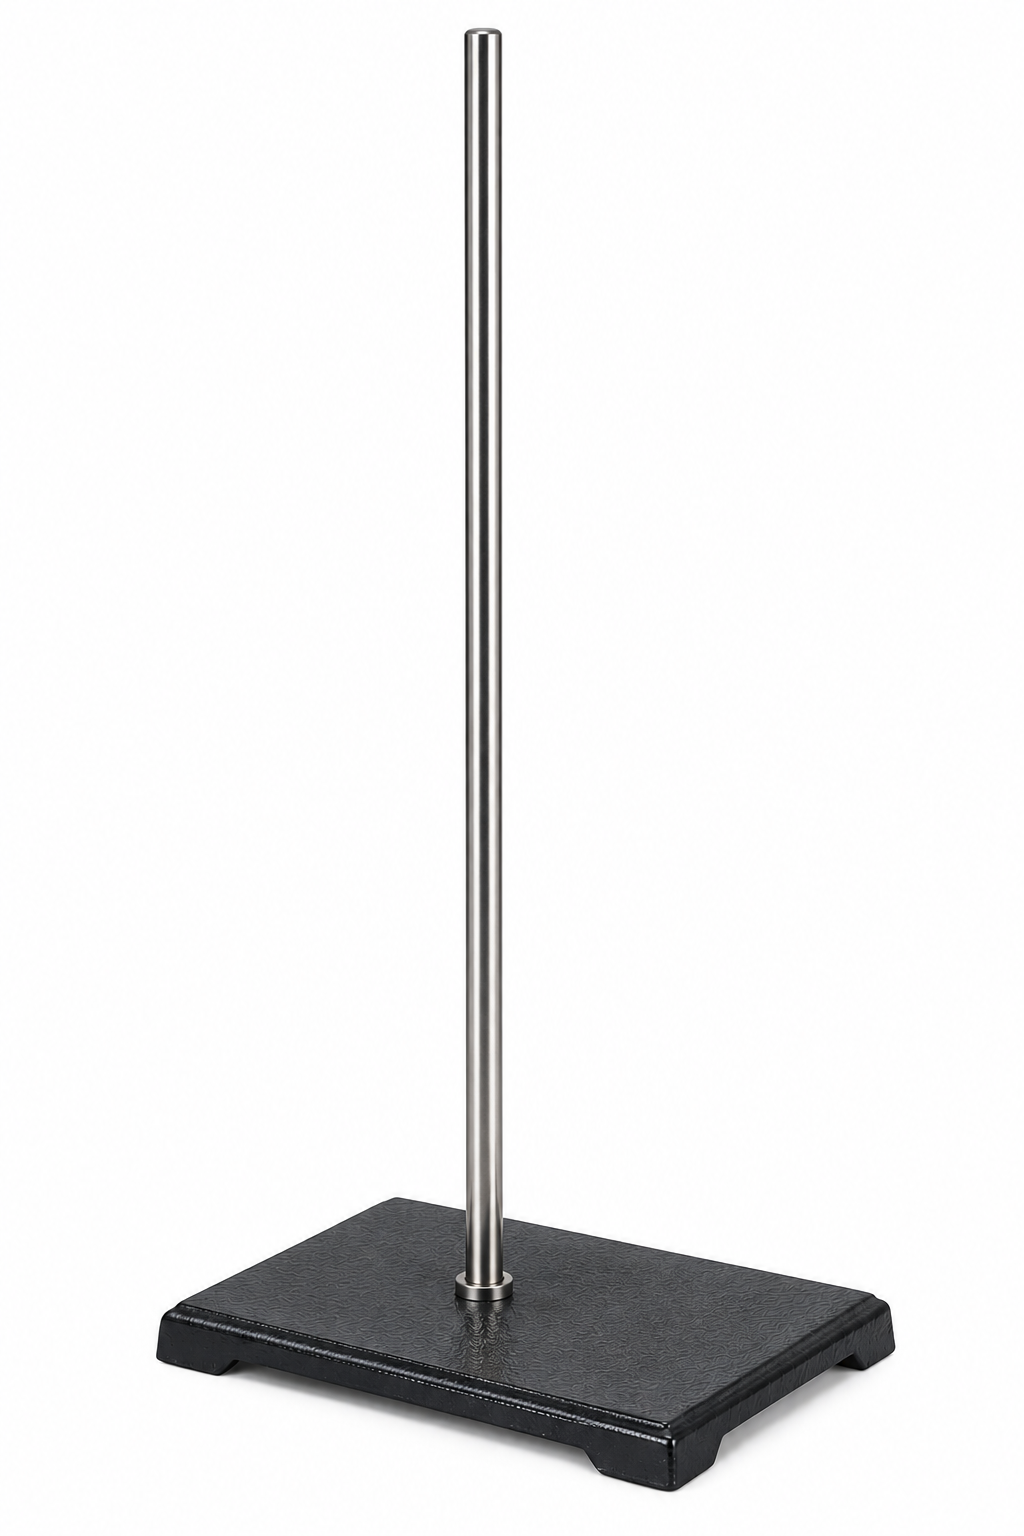
\includegraphics[width=0.38\textwidth]{../figuras/soporte_universal.png}

    \vspace{0.2cm}

    \textbf{Figura 1.} Soporte universal empleado en el montaje experimental.
\end{center}

\end{list}

% ------------------------------------------------------------
% 4.1.2 BARRA METÁLICA DE SOPORTE
% ------------------------------------------------------------

\begin{list}{}{\leftmargin=1.2cm\rightmargin=0cm}
\item[]

\textbf{4.1.2. Barra metálica de soporte}

\vspace{0.3em}

Barra metálica empleada como elemento auxiliar del soporte universal para
sostener y posicionar los componentes del montaje experimental mediante
las nueces de sujeción.

\begin{itemize}
    \item \textbf{Material:} Metálico.
    \item \textbf{Función:} Sujeción y posicionamiento de los componentes
    del sistema.
\end{itemize}

\begin{center}
    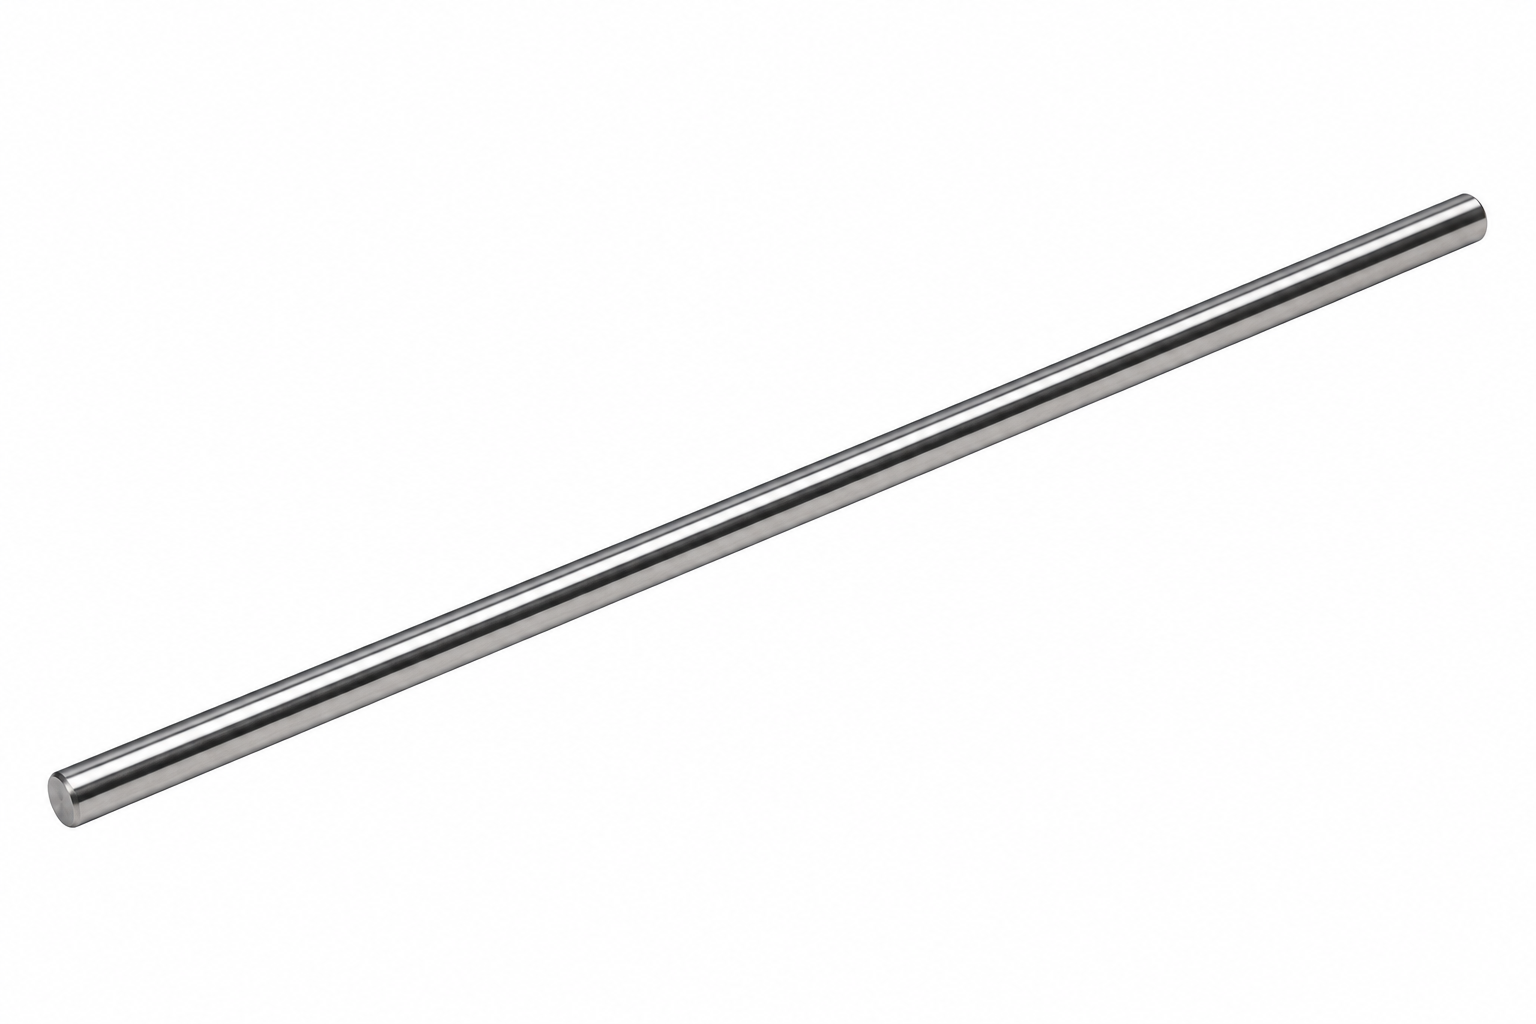
\includegraphics[width=0.48\textwidth]{../figuras/barra_metalica.png}

    \vspace{0.2cm}

    \textbf{Figura 2.} Barra metálica empleada como elemento de soporte
    en el montaje experimental.
\end{center}

\end{list}

% ------------------------------------------------------------
% 4.1.3 NUECES DOBLES DE SUJECIÓN
% ------------------------------------------------------------

\begin{list}{}{\leftmargin=1.2cm\rightmargin=0cm}
\item[]

\textbf{4.1.3. Nueces dobles de sujeción}

\vspace{0.3em}

Elementos de fijación empleados para unir la barra metálica al soporte
universal y mantener los componentes del montaje en una posición estable
durante la experiencia.

\begin{itemize}
    \item \textbf{Cantidad:} 2 unidades.
    \item \textbf{Material:} Metálico.
    \item \textbf{Función:} Unión y fijación de los elementos del montaje.
\end{itemize}

\begin{center}
    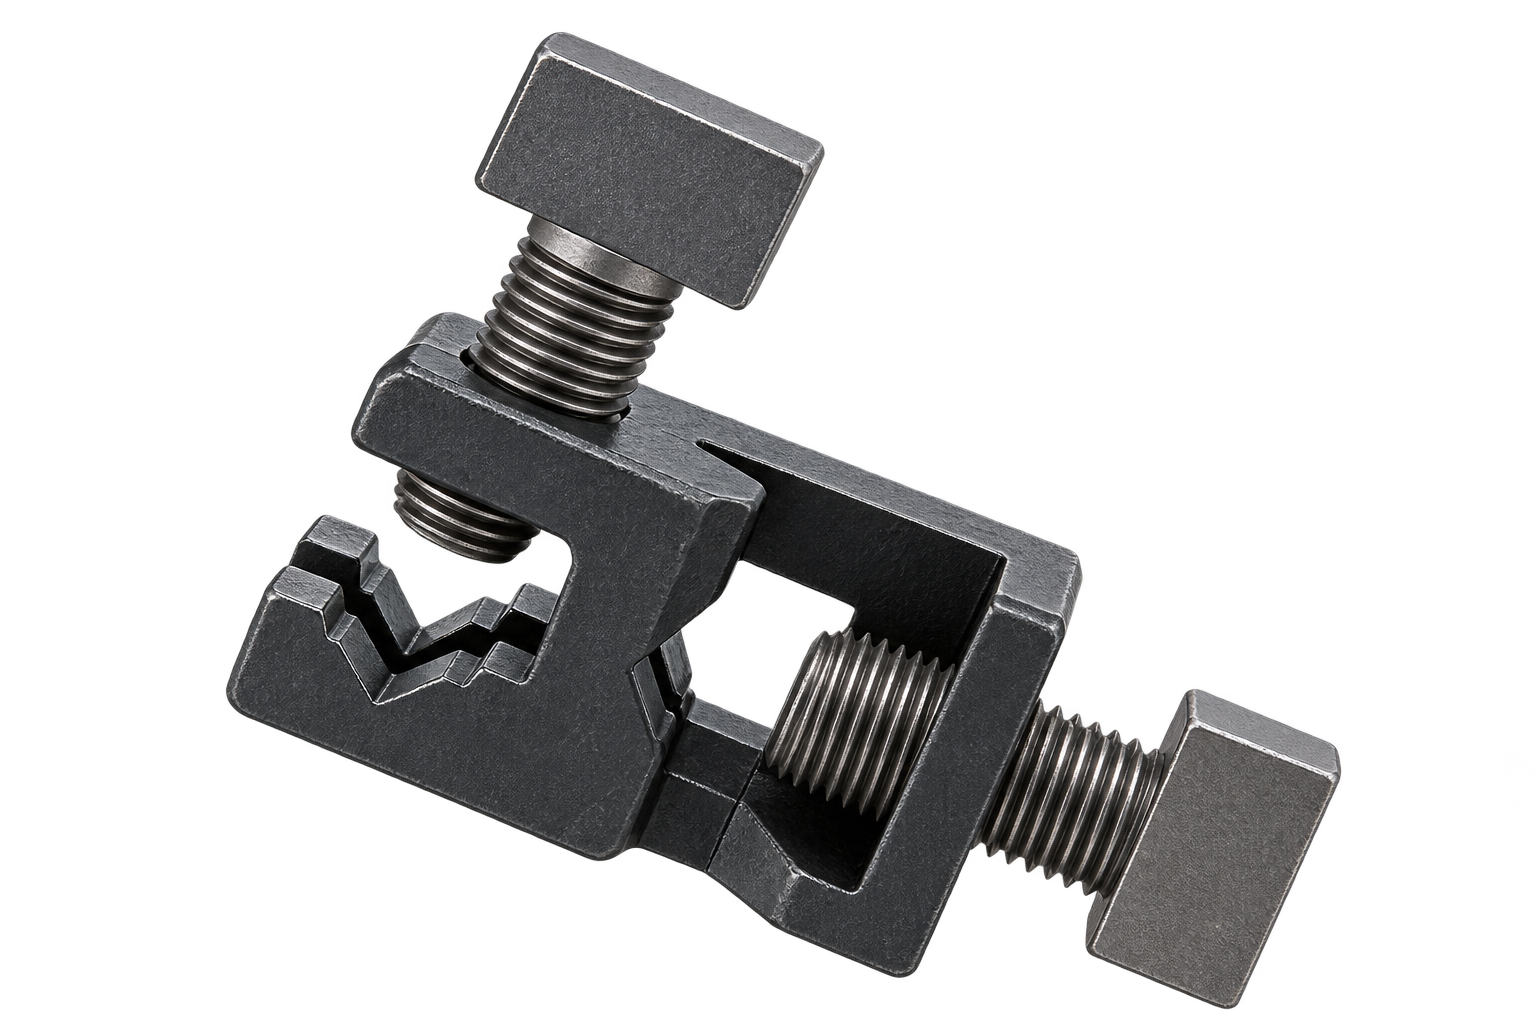
\includegraphics[width=0.45\textwidth]{../figuras/nuez.png}

    \vspace{0.2cm}

    \textbf{Figura 3.} Nueces dobles de sujeción empleadas en el montaje
    experimental.
\end{center}

\end{list}

% ============================================================
% 4.2 INSTRUMENTOS DE MEDICIÓN Y ADQUISICIÓN DE DATOS
% ============================================================

\subsection*{4.2. Instrumentos de medición y adquisición de datos}

% ------------------------------------------------------------
% 4.2.1 CALIBRADOR VERNIER
% ------------------------------------------------------------

\begin{list}{}{\leftmargin=1.2cm\rightmargin=0cm}
\item[]

\textbf{4.2.1. Calibrador Vernier}

\vspace{0.3em}

Instrumento de medición dimensional empleado para determinar con precisión
los diámetros y dimensiones geométricas de los componentes del sistema
rotacional.

\begin{itemize}
    \item \textbf{Tipo:} Analógico.
    \item \textbf{Resolución:} \(0.05\,\mathrm{mm}\).
    \item \textbf{Función:} Medición de los diámetros del disco, anillo y
    cilindro del sistema rotacional.
\end{itemize}

\begin{center}
    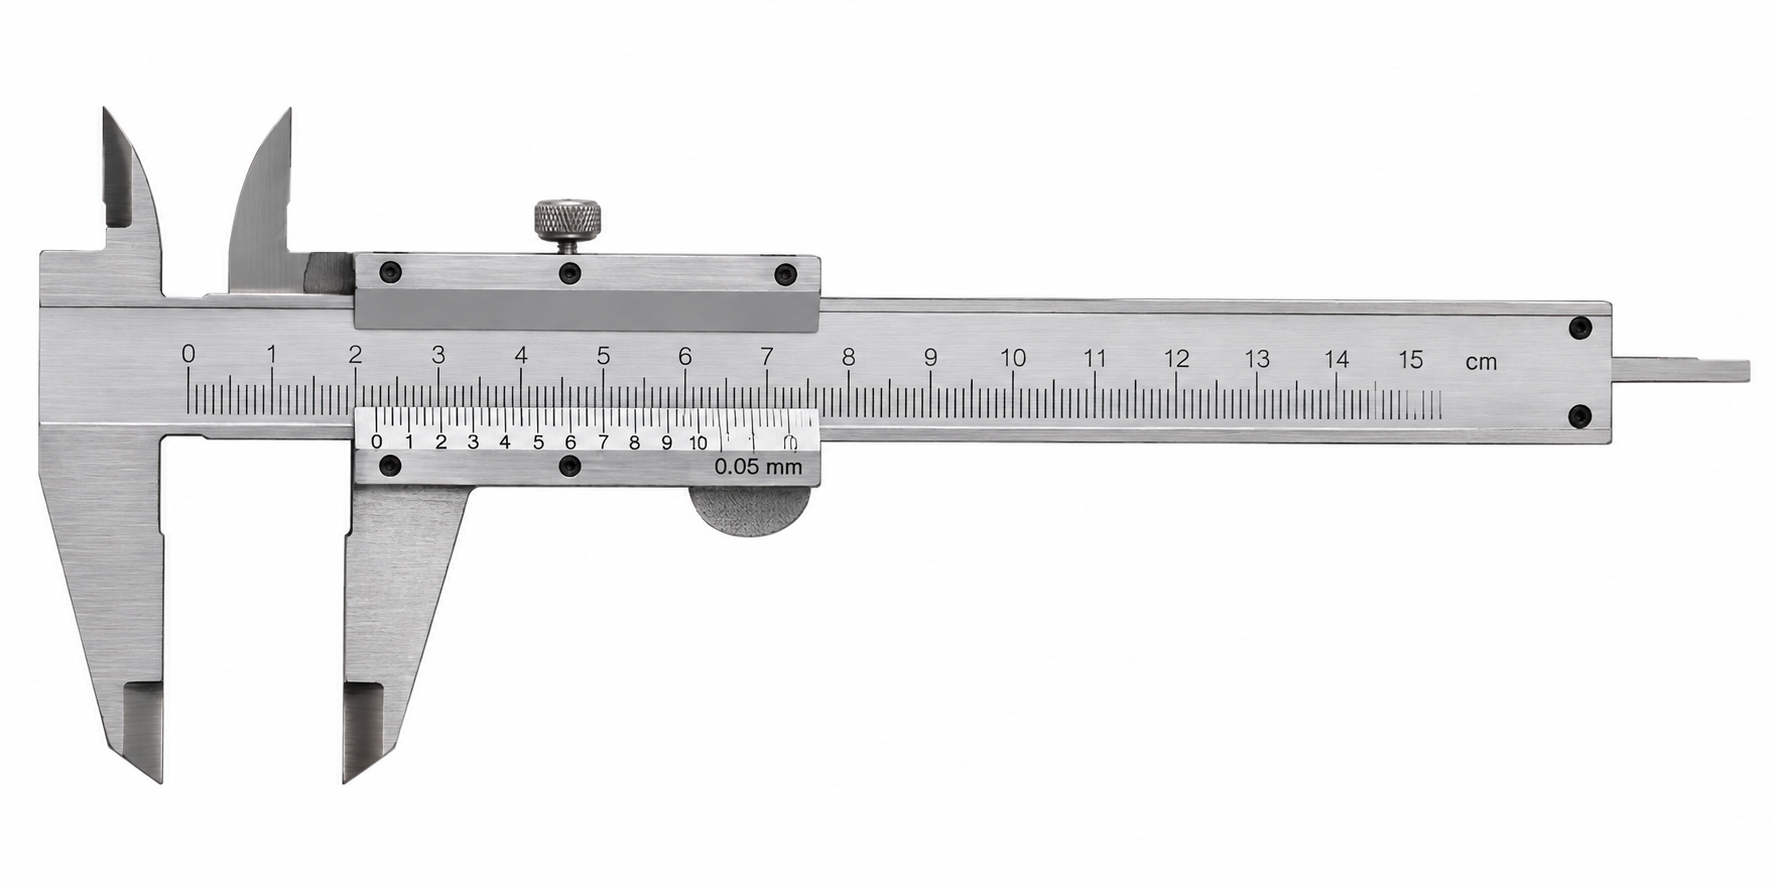
\includegraphics[width=0.60\textwidth]{../figuras/vernier.png}

    \vspace{0.2cm}

    \textbf{Figura 4.} Calibrador Vernier empleado para la medición de las
    dimensiones geométricas del sistema.
\end{center}

\end{list}

% ------------------------------------------------------------
% 4.2.2 BALANZA DIGITAL
% ------------------------------------------------------------

\begin{list}{}{\leftmargin=1.2cm\rightmargin=0cm}
\item[]

\textbf{4.2.2. Balanza digital}

\vspace{0.3em}

Instrumento empleado para determinar la masa del disco, del anillo y de
los elementos que conforman la masa suspendida, magnitudes necesarias para
el cálculo de los momentos de inercia teóricos y experimentales.

\begin{itemize}
    \item \textbf{Tipo:} Digital.
    \item \textbf{Resolución:} \(0.1\,\mathrm{g}\).
    \item \textbf{Función:} Medición de las masas de los componentes
    utilizados en el sistema experimental.
\end{itemize}

\begin{center}
    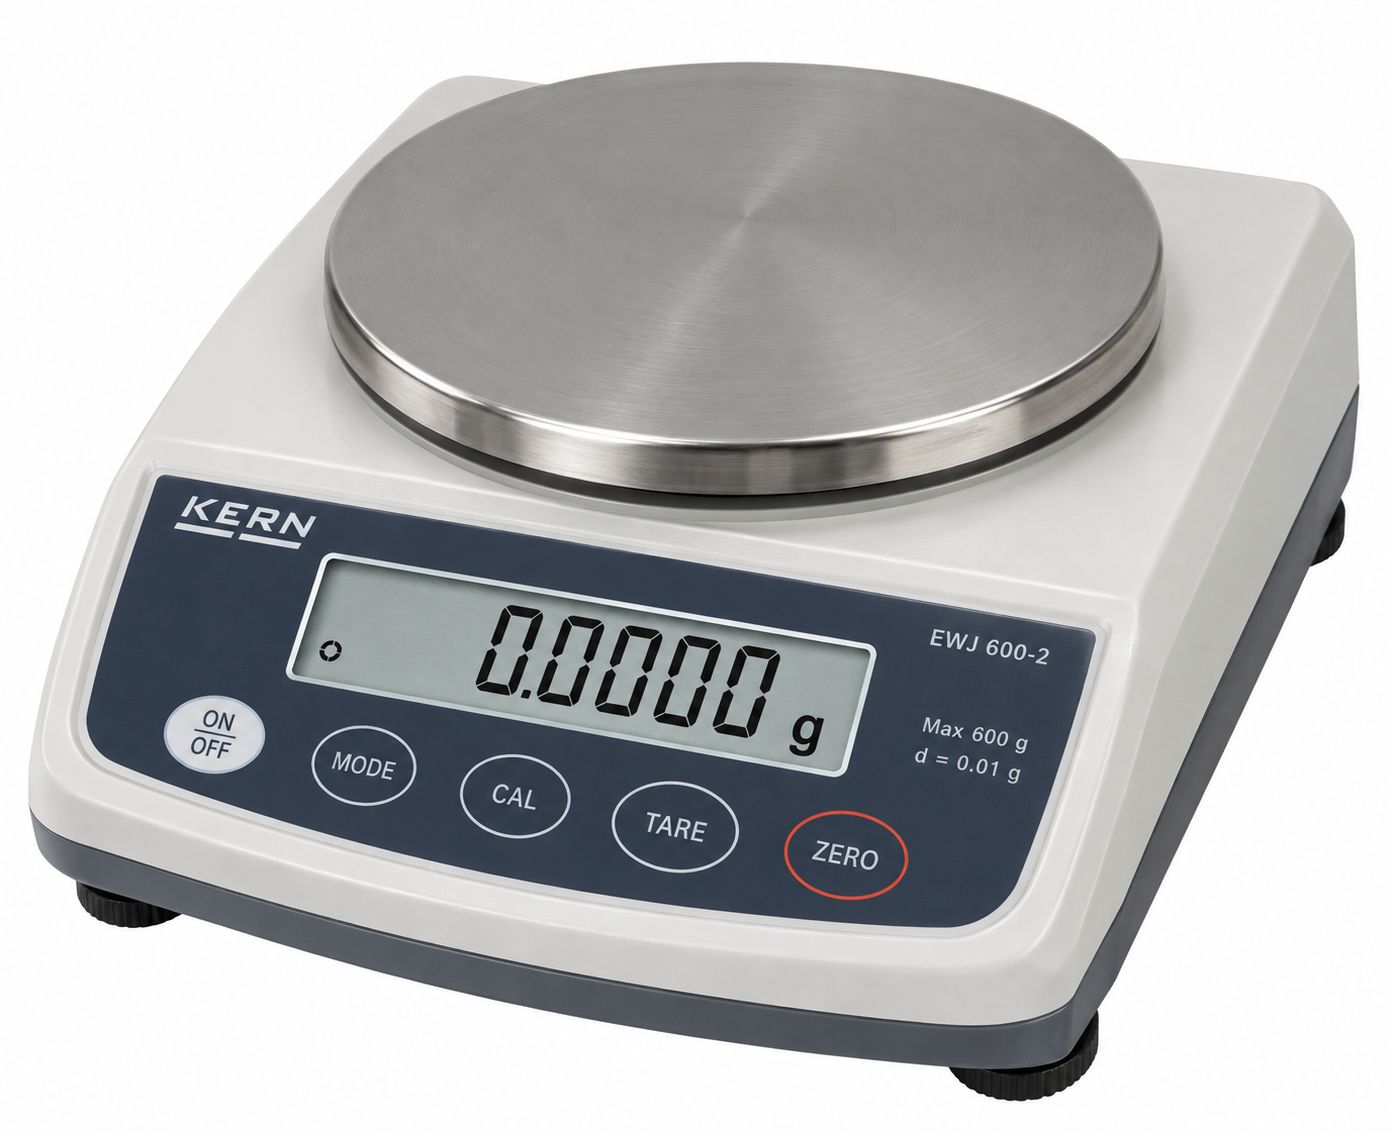
\includegraphics[width=0.43\textwidth]{../figuras/balanza.png}

    \vspace{0.2cm}

    \textbf{Figura 5.} Balanza digital empleada para la medición de las
    masas de los componentes del sistema experimental.
\end{center}

\end{list}

% ------------------------------------------------------------
% 4.2.3 FOTOPUERTA (LIGHT GATE)
% ------------------------------------------------------------

\begin{list}{}{\leftmargin=1.2cm\rightmargin=0cm}
\item[]

\textbf{4.2.3. Fotopuerta (Light Gate)}

\vspace{0.3em}

Sensor fotoeléctrico empleado para registrar el movimiento del sistema
durante la experiencia. Los datos obtenidos permitieron determinar la
velocidad en función del tiempo y, mediante un ajuste lineal, calcular
la aceleración de la masa suspendida.

\begin{itemize}
    \item \textbf{Tipo:} sensor fotoeléctrico digital.
    \item \textbf{Magnitud registrada:} tiempo de paso y movimiento del sistema.
    \item \textbf{Función:} adquisición de los datos necesarios para obtener
    la gráfica de velocidad en función del tiempo.
\end{itemize}

\begin{center}
    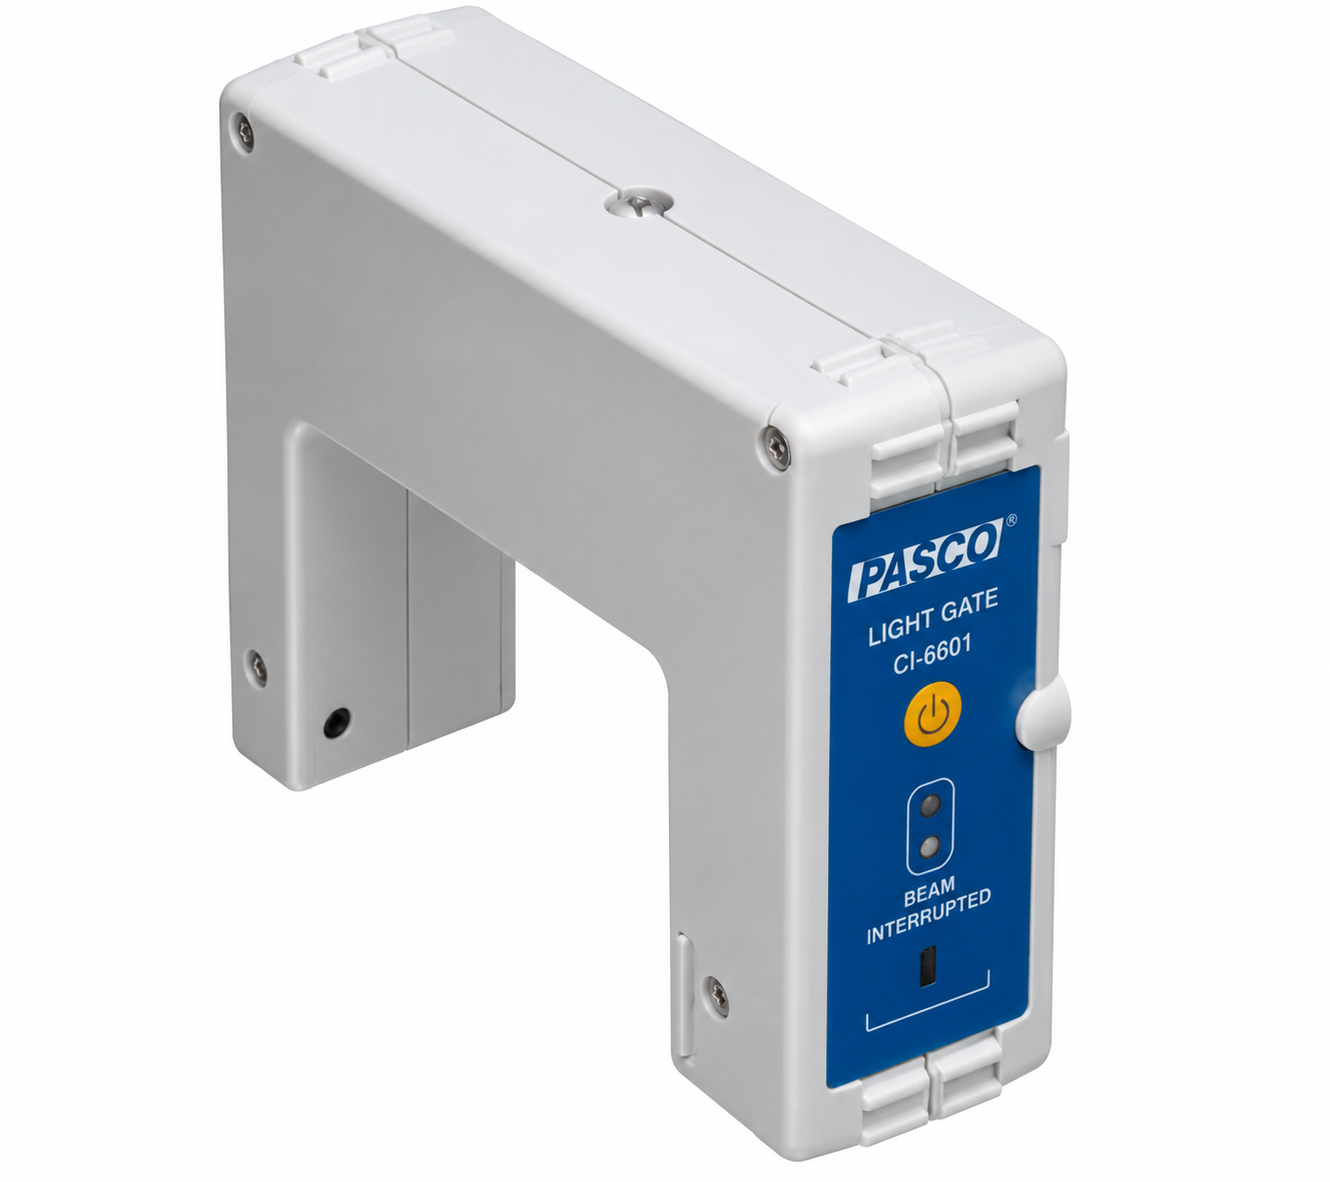
\includegraphics[width=0.38\textwidth]{../figuras/light_gate.png}

    \vspace{0.2cm}

    \textbf{Figura 6.} Fotopuerta (Light Gate) empleada para la adquisición
    de datos del movimiento del sistema.
\end{center}

\end{list}

% ============================================================
% 4.3 COMPONENTES DEL SISTEMA ROTACIONAL
% ============================================================

\subsection*{4.3. Componentes del sistema rotacional}

% ------------------------------------------------------------
% 4.3.1 BASE DEL SISTEMA ROTACIONAL
% ------------------------------------------------------------

\begin{list}{}{\leftmargin=1.2cm\rightmargin=0cm}
\item[]

\textbf{4.3.1. Base del sistema rotacional}

\vspace{0.3em}

Estructura metálica que constituye el soporte principal del sistema
rotacional. Sobre ella se encuentra dispuesto el eje de rotación que
permite el montaje y giro del conjunto disco--anillo durante la
experiencia.

\begin{itemize}
    \item \textbf{Material:} metálico.
    \item \textbf{Función:} soporte y estabilización del sistema rotacional.
\end{itemize}

\begin{center}
    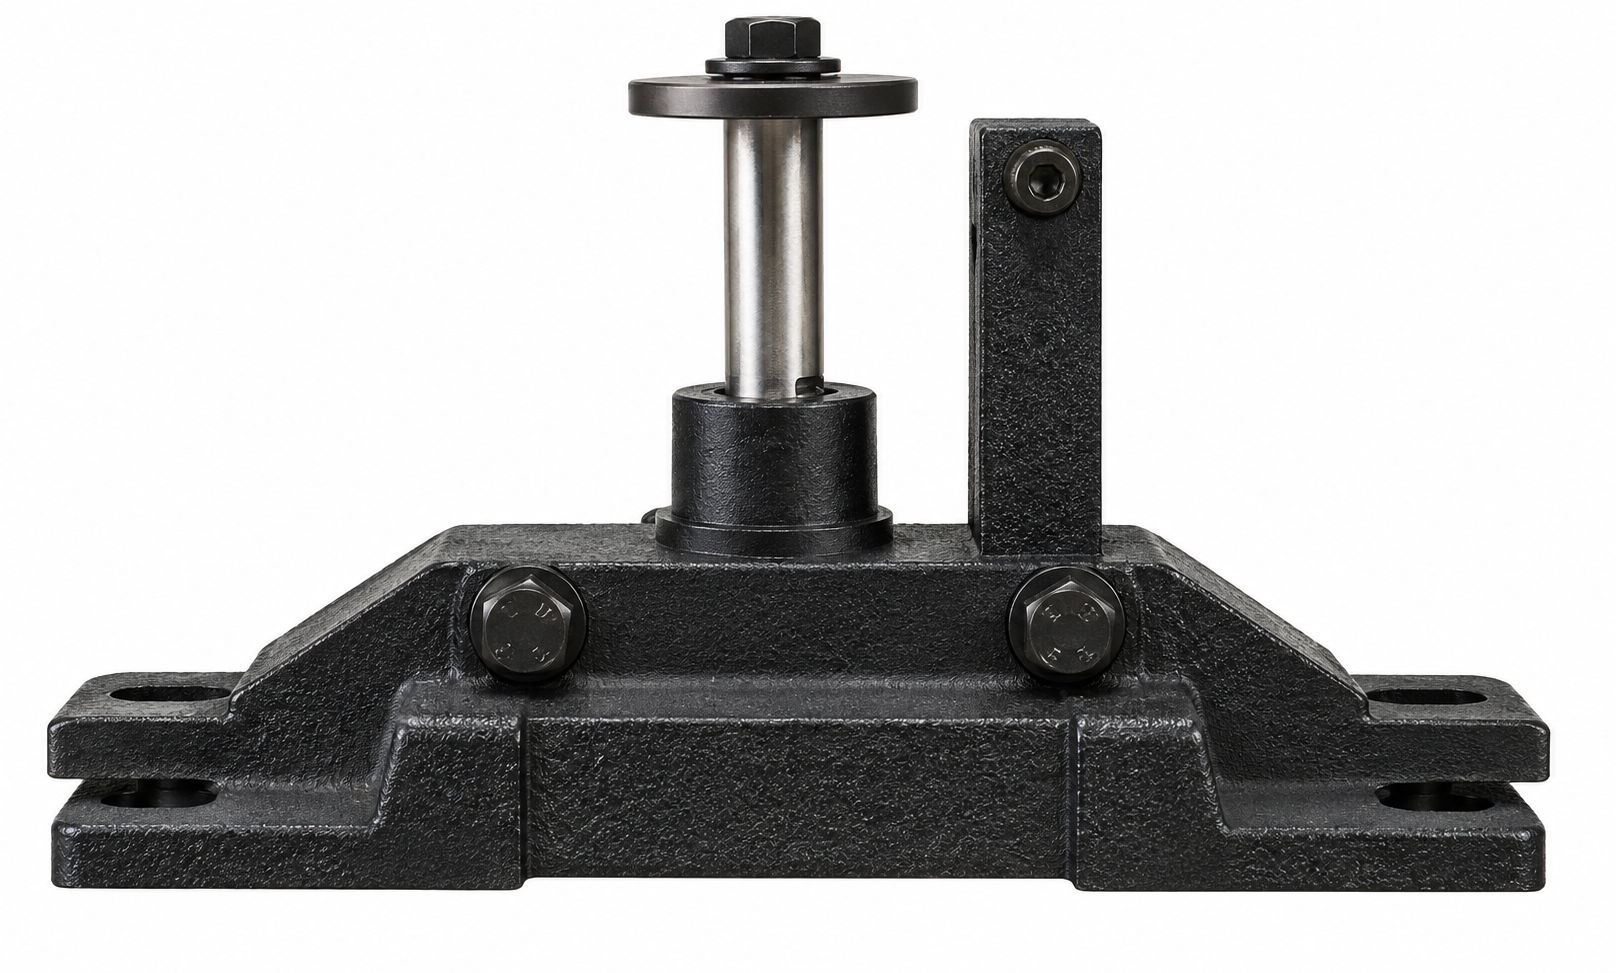
\includegraphics[width=0.48\textwidth]{../figuras/base.png}

    \vspace{0.2cm}

    \textbf{Figura 7.} Base empleada como soporte del sistema rotacional.
\end{center}

\end{list}

% ------------------------------------------------------------
% 4.3.2 CONJUNTO DISCO--ANILLO
% ------------------------------------------------------------

\begin{list}{}{\leftmargin=1.2cm\rightmargin=0cm}
\item[]

\textbf{4.3.2. Conjunto disco--anillo}

\vspace{0.3em}

Conjunto de cuerpos metálicos constituido por un disco y un anillo
homogéneos, dispuestos coaxialmente sobre el eje de rotación. Sus masas
y dimensiones geométricas se emplearon para determinar y comparar sus
momentos de inercia teóricos y experimentales.

\begin{itemize}
    \item \textbf{Material:} metálico.
    \item \textbf{Componentes:} disco y anillo.
    \item \textbf{Función:} cuerpos de estudio para la determinación
    experimental del momento de inercia.
\end{itemize}

\begin{center}
    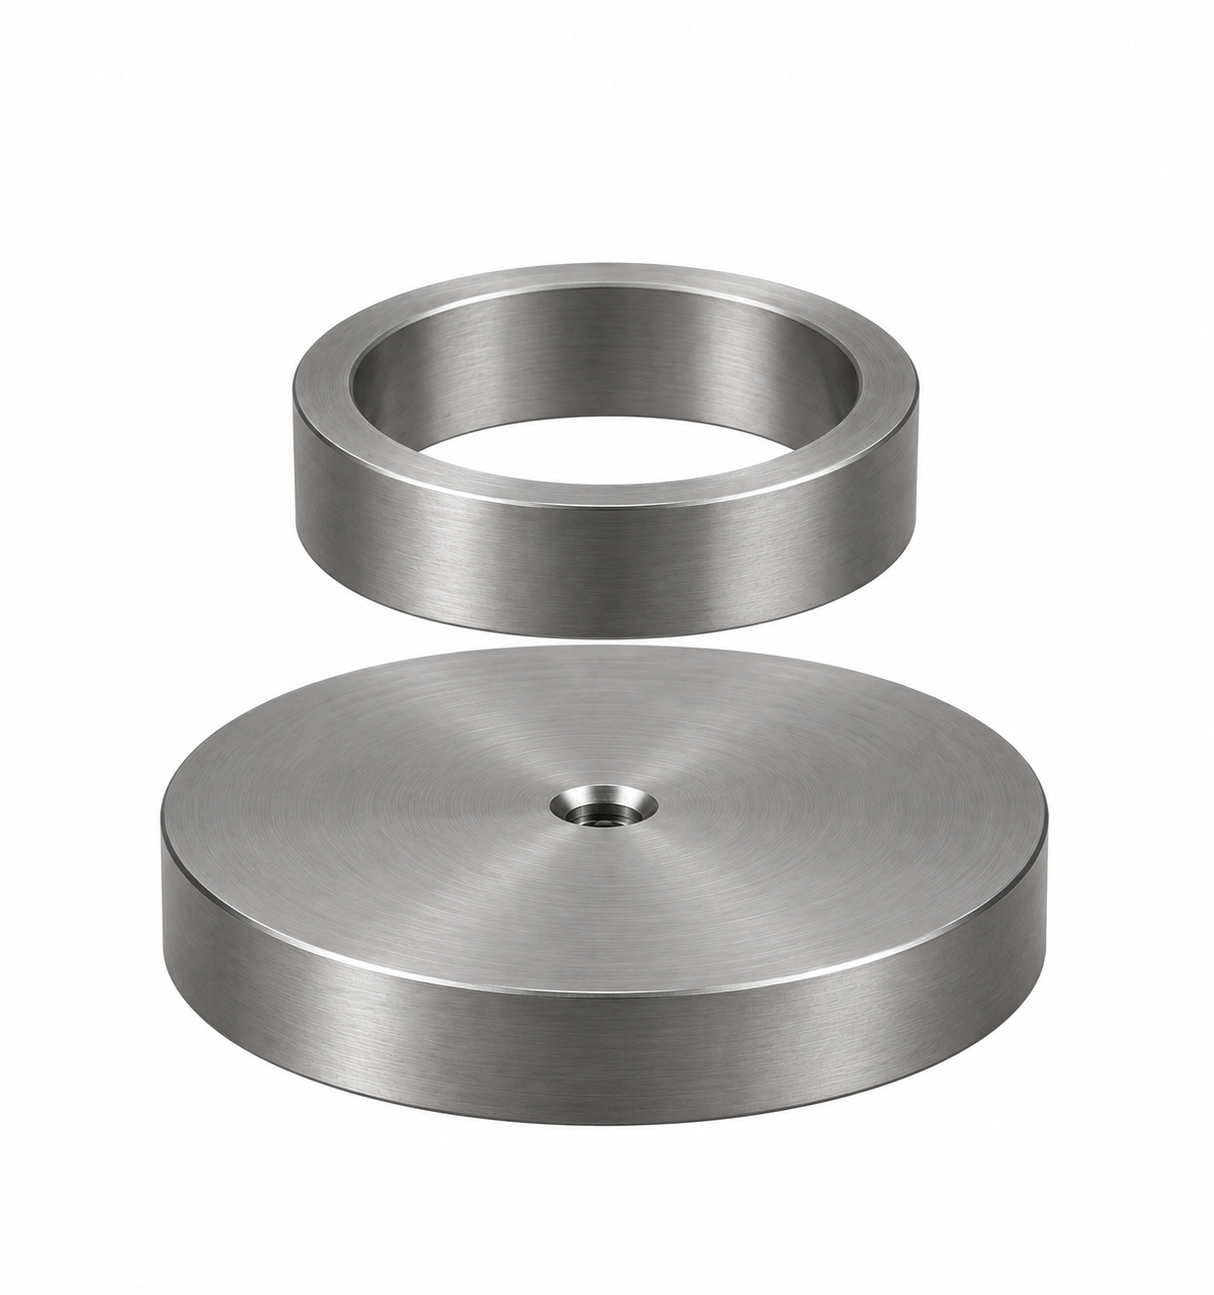
\includegraphics[width=0.48\textwidth]{../figuras/disco_anillo.png}

    \vspace{0.2cm}

    \textbf{Figura 8.} Disco y anillo empleados en la determinación
    experimental del momento de inercia.
\end{center}

\end{list}

% ------------------------------------------------------------
% 4.3.3 SISTEMA POLEA--HILO
% ------------------------------------------------------------

\begin{list}{}{\leftmargin=1.2cm\rightmargin=0cm}
\item[]

\textbf{4.3.3. Sistema polea--hilo}

\vspace{0.3em}

Sistema constituido por una polea de plástico y un hilo que conecta el
sistema rotacional con la masa suspendida. El hilo transmite la tensión
generada durante el descenso de la masa, permitiendo producir el movimiento
del sistema.

\begin{itemize}
    \item \textbf{Material de la polea:} plástico.
    \item \textbf{Componentes:} polea e hilo.
    \item \textbf{Función:} transmisión del movimiento entre el sistema
    rotacional y la masa suspendida.
\end{itemize}

\begin{center}
    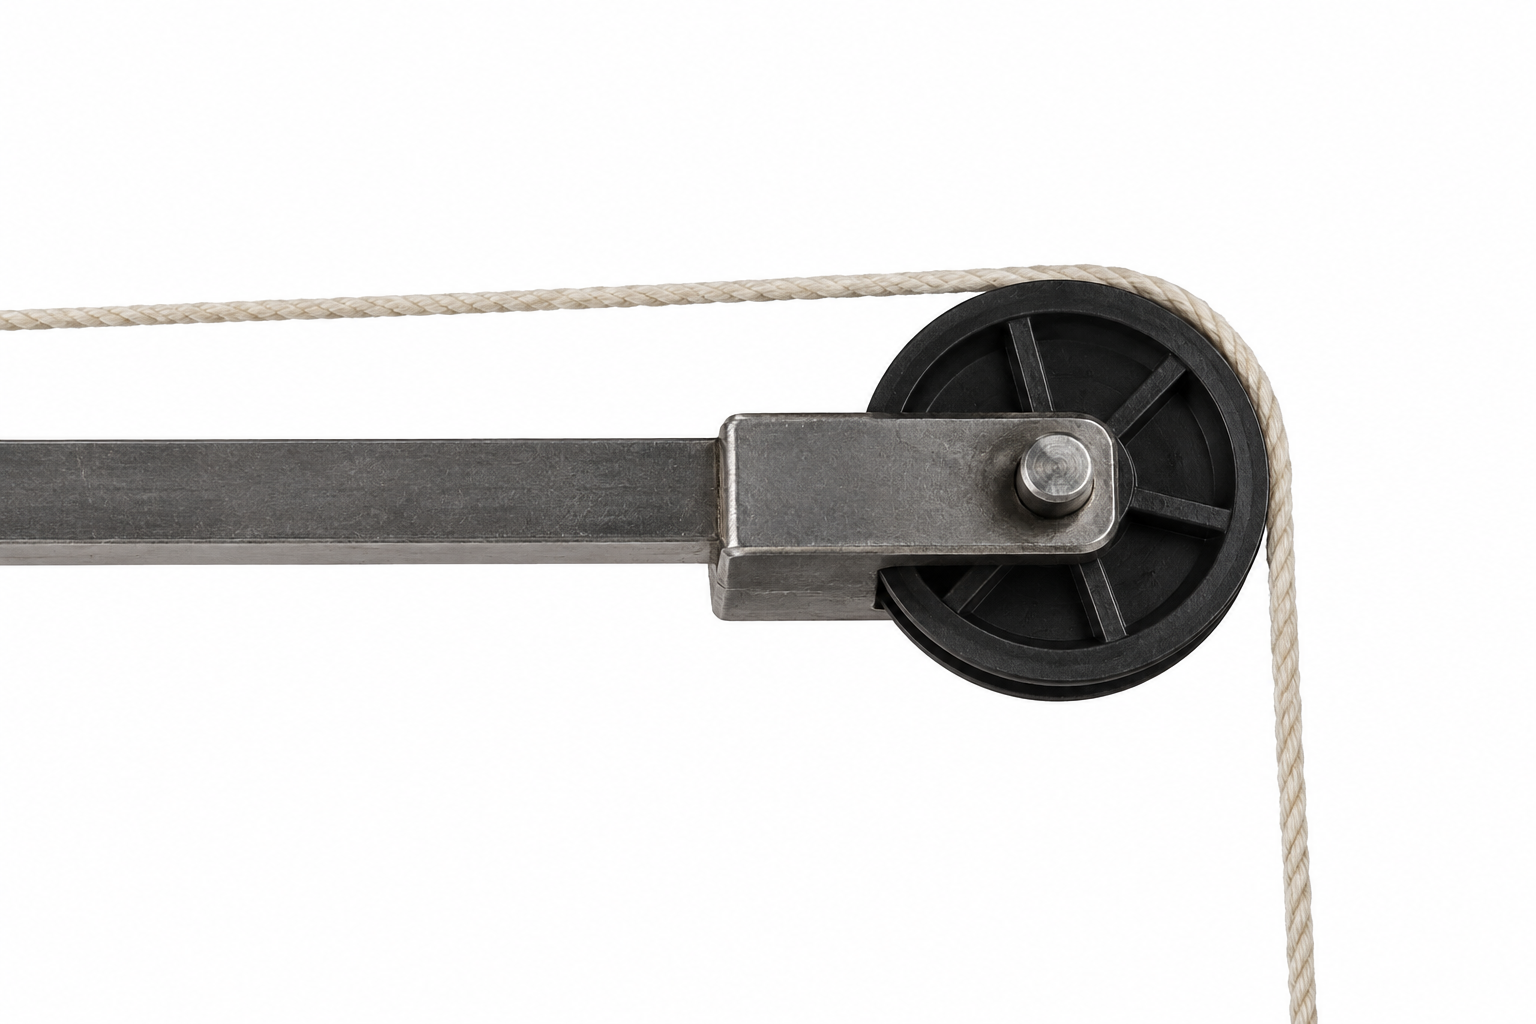
\includegraphics[width=0.50\textwidth]{../figuras/polea.png}

    \vspace{0.2cm}

    \textbf{Figura 9.} Sistema polea--hilo empleado en el montaje experimental.
\end{center}

\end{list}

% ------------------------------------------------------------
% 4.3.4 PORTAPESAS Y MASA SUSPENDIDA
% ------------------------------------------------------------

\begin{list}{}{\leftmargin=1.2cm\rightmargin=0cm}
\item[]

\textbf{4.3.4. Portapesas y masa suspendida}

\vspace{0.3em}

Conjunto formado por un portapesas de plástico conectado al hilo y por
pesas metálicas. Durante el experimento, su descenso proporciona la fuerza
necesaria para producir la rotación del sistema disco--anillo.

\begin{itemize}
    \item \textbf{Material del portapesas:} plástico.
    \item \textbf{Material de las pesas:} metálico.
    \item \textbf{Función:} generar, mediante su peso, el movimiento del
    sistema rotacional.
\end{itemize}

\begin{center}
    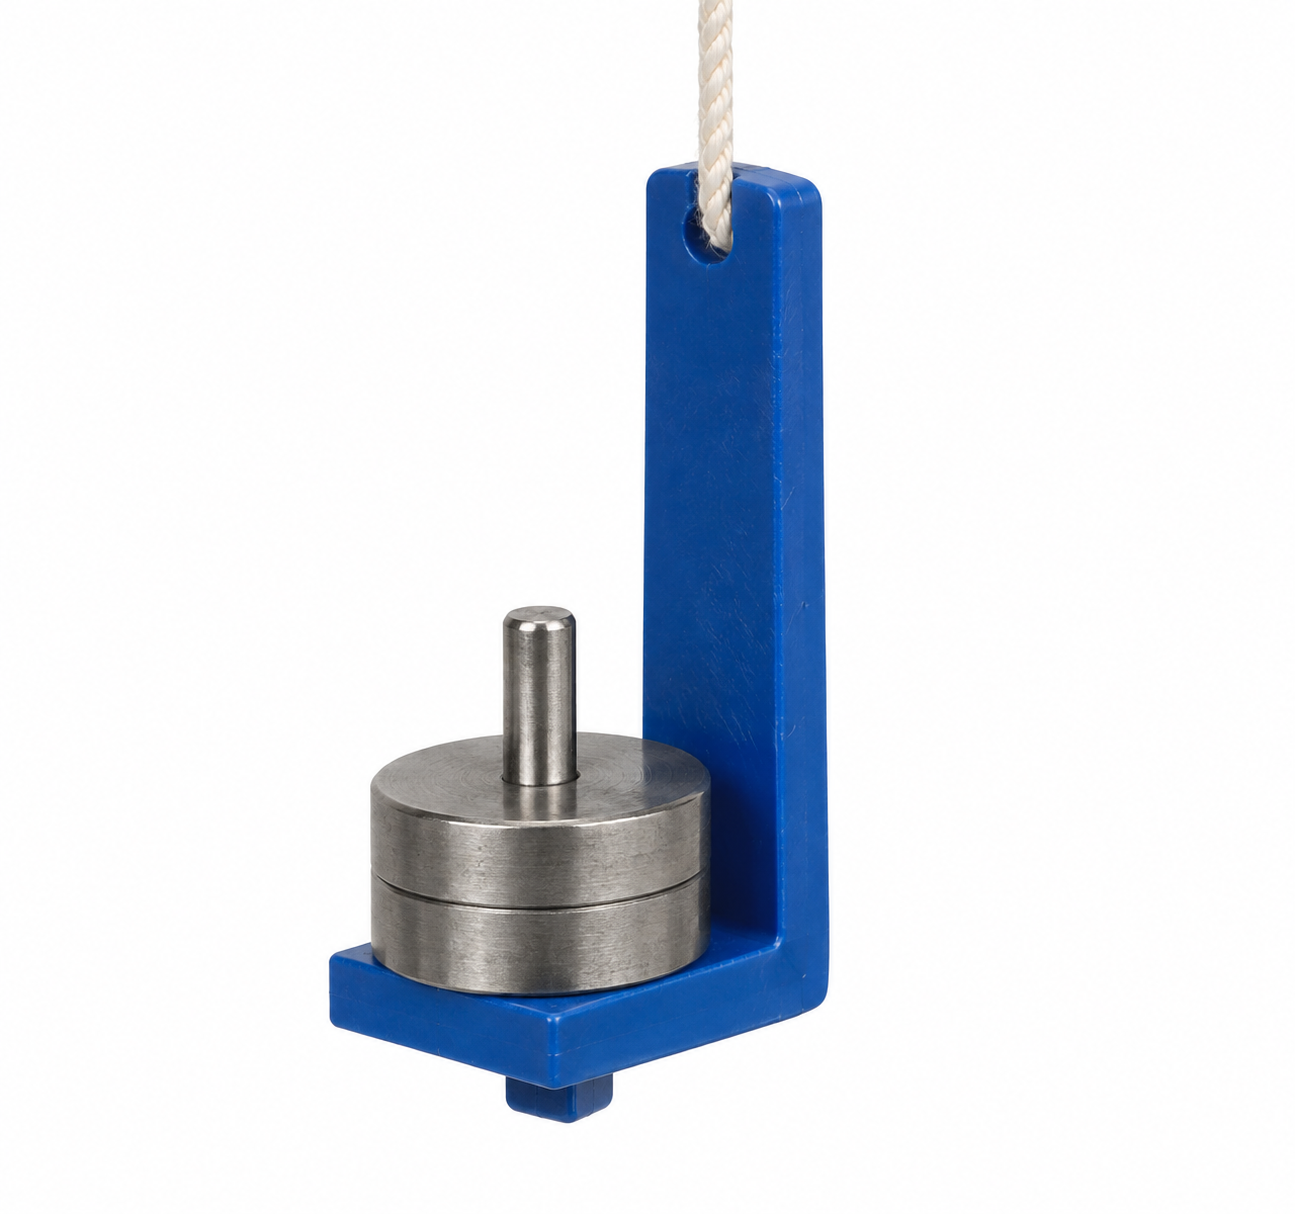
\includegraphics[width=0.38\textwidth]{../figuras/colgador.png}

    \vspace{0.2cm}

    \textbf{Figura 10.} Portapesas y masas suspendidas empleadas en el
    sistema experimental.
\end{center}

\end{list}

% ============================================================
% 5. PROCEDIMIENTO EXPERIMENTAL
% ============================================================

\newpage

\section*{5. PROCEDIMIENTO EXPERIMENTAL}
\addcontentsline{toc}{section}{5. PROCEDIMIENTO EXPERIMENTAL}
\sectionline

% ------------------------------------------------------------
% 5.1 MEDICIÓN DE LAS CARACTERÍSTICAS DEL DISCO Y DEL ANILLO
% ------------------------------------------------------------

\subsection*{5.1. Medición de las características del disco y del anillo}

Inicialmente, se determinaron las magnitudes necesarias para el cálculo
teórico del momento de inercia de los cuerpos empleados. Mediante la
balanza digital se midieron las masas del disco y del anillo, mientras
que con el calibrador Vernier se determinaron sus dimensiones geométricas.

Para el disco se midió su diámetro exterior. En el caso del anillo, se
midieron tanto el diámetro interior como el diámetro exterior. Cada
magnitud fue registrada junto con la incertidumbre correspondiente al
instrumento utilizado.

De esta manera se obtuvieron las magnitudes \(M_D\), \(D_D\), \(M_A\),
\(D_i\) y \(D_e\), que posteriormente se emplearon para calcular los
momentos de inercia teóricos del disco y del anillo.


% ------------------------------------------------------------
% 5.2 MONTAJE DEL SISTEMA EXPERIMENTAL
% ------------------------------------------------------------

\subsection*{5.2. Montaje del sistema experimental}

Se instaló la base del sistema rotacional sobre la mesa de trabajo y se
dispuso el disco sobre su eje de rotación. Posteriormente, se colocó el
anillo sobre el disco de manera que ambos cuerpos permanecieran
aproximadamente coaxiales.

A continuación, se colocó el hilo alrededor del cilindro solidario al
eje del sistema rotacional y se hizo pasar su extremo libre por la polea.
En dicho extremo se conectó el portapesas con la masa suspendida, de modo
que su descenso produjera una tensión en el hilo y, en consecuencia, un
torque sobre el eje del sistema.

La polea y los elementos auxiliares se fijaron mediante el soporte
universal, la barra metálica y las nueces de sujeción. Finalmente, se
posicionó la fotopuerta (\textit{Light Gate}) de manera adecuada para
registrar el movimiento asociado al descenso de la masa suspendida.


% ------------------------------------------------------------
% 5.3 MEDICIÓN DE LOS PARÁMETROS DEL SISTEMA
% ------------------------------------------------------------

\subsection*{5.3. Medición de los parámetros del sistema}

Antes de iniciar la adquisición de datos dinámicos, se midió con el
calibrador Vernier el diámetro \(d\) del cilindro sobre el cual se
enrollaba el hilo. Esta dimensión determina el radio efectivo de
aplicación de la tensión y, por tanto, interviene directamente en el
cálculo experimental del momento de inercia.

Asimismo, mediante la balanza digital se determinó la masa total
suspendida \(m\), considerando el conjunto formado por el portapesas y
las masas colocadas sobre este. Tanto el diámetro del cilindro como la
masa suspendida se registraron con sus respectivas incertidumbres
experimentales.


% ------------------------------------------------------------
% 5.4 ADQUISICIÓN DE DATOS DEL SISTEMA DISCO--ANILLO
% ------------------------------------------------------------

\subsection*{5.4. Adquisición de datos del sistema disco--anillo}

Con el disco y el anillo colocados sobre el eje de rotación, se enrolló
el hilo alrededor del cilindro y se elevó la masa suspendida hasta la
posición inicial establecida. Se verificó que el hilo permaneciera
correctamente dispuesto sobre la polea y que la masa pudiera descender
sin obstáculos.

Seguidamente, se liberó la masa suspendida desde el reposo, permitiendo
que descendiera bajo la acción de la gravedad. La tensión producida en
el hilo generó un torque sobre el eje y provocó la rotación conjunta del
disco y del anillo.

Durante el movimiento, la fotopuerta registró los datos necesarios para
obtener la velocidad del sistema en función del tiempo. Los valores
registrados se almacenaron para su posterior procesamiento y análisis.


% ------------------------------------------------------------
% 5.5 ADQUISICIÓN DE DATOS DEL DISCO
% ------------------------------------------------------------

\subsection*{5.5. Adquisición de datos del disco}

Finalizada la medición correspondiente al sistema disco--anillo, se
retiró cuidadosamente el anillo, manteniendo el disco sobre el mismo eje
de rotación y conservando la configuración general del montaje
experimental.

Se volvió a enrollar el hilo alrededor del cilindro y se colocó la masa
suspendida en la posición inicial. Posteriormente, se liberó nuevamente
la masa desde el reposo y se registró el movimiento mediante la
fotopuerta.

De esta forma se obtuvieron los datos de velocidad en función del tiempo
correspondientes al movimiento del disco sin el anillo, necesarios para
determinar experimentalmente su momento de inercia.


% ------------------------------------------------------------
% 5.6 PROCESAMIENTO DE LOS DATOS EXPERIMENTALES
% ------------------------------------------------------------

\subsection*{5.6. Procesamiento de los datos experimentales}

Los datos obtenidos mediante la fotopuerta fueron organizados para
construir las gráficas de velocidad en función del tiempo,
\(v(t)\), correspondientes a las configuraciones disco--anillo y disco.

Para cada conjunto de datos se realizó un ajuste lineal de acuerdo con
la expresión del movimiento uniformemente acelerado,

\[
v(t)=v_0+at,
\]

donde la pendiente de la recta representa la aceleración lineal \(a\)
del sistema. A partir de las pendientes obtenidas y de los parámetros
medidos previamente, se determinaron posteriormente los momentos de
inercia experimentales.

Finalmente, el momento de inercia experimental del anillo se obtuvo a
partir de la diferencia entre el momento de inercia del sistema
disco--anillo y el correspondiente al disco. Los valores experimentales
fueron comparados posteriormente con los valores teóricos calculados a
partir de las masas y dimensiones geométricas de ambos cuerpos.

% ============================================================
% 6. RESULTADOS EXPERIMENTALES
% ============================================================

\newpage

\section*{6. RESULTADOS EXPERIMENTALES}
\addcontentsline{toc}{section}{6. RESULTADOS EXPERIMENTALES}
\sectionline

En esta sección se presentan los datos experimentales obtenidos durante
la experiencia para la determinación del momento de inercia del disco y
del anillo. Se incluyen las mediciones de masa y dimensiones geométricas
de los cuerpos, los parámetros correspondientes al sistema rotacional y
los registros de tiempo y velocidad obtenidos mediante la fotopuerta.
Todas las magnitudes medidas directamente se expresan en unidades del
Sistema Internacional y se presentan junto con sus respectivas
incertidumbres experimentales.

La Tabla 1 reúne las masas y dimensiones geométricas del disco y del
anillo. Estas magnitudes se mantuvieron constantes durante la experiencia
y serán empleadas posteriormente para la determinación de los momentos
de inercia teóricos.

\begin{table}[h!]
\centering
\renewcommand{\arraystretch}{1.25}

\begin{tabular}{lcc}
\hline
\textbf{Magnitud} & \textbf{Símbolo} & \textbf{Valor} \\
\hline
Masa del disco
& \(M_D\)
& \((1.4544 \pm 0.0001)\,\mathrm{kg}\) \\

Radio del disco
& \(R_D\)
& \((0.11430 \pm 0.00050)\,\mathrm{m}\) \\

Masa del anillo
& \(M_A\)
& \((1.4466 \pm 0.0001)\,\mathrm{kg}\) \\

Radio interior del anillo
& \(R_i\)
& \((0.053575 \pm 0.000050)\,\mathrm{m}\) \\

Radio exterior del anillo
& \(R_e\)
& \((0.063825 \pm 0.000050)\,\mathrm{m}\) \\
\hline
\end{tabular}

\vspace{0.2cm}

\textbf{Cuadro 1:} Características experimentales del disco y del anillo.

\end{table}


La Tabla 2 presenta los parámetros correspondientes al montaje
rotacional utilizados durante la adquisición de datos. Se incluye el
diámetro del cilindro sobre el cual se enrolló el hilo y la masa total
suspendida, considerando tanto el portapesas como las masas colocadas
sobre este.

\begin{table}[h!]
\centering
\renewcommand{\arraystretch}{1.25}

\begin{tabular}{lcc}
\hline
\textbf{Magnitud} & \textbf{Símbolo} & \textbf{Valor} \\
\hline
Diámetro del cilindro
& \(d\)
& \((0.01310 \pm 0.00005)\,\mathrm{m}\) \\

Masa total suspendida
& \(m\)
& \((0.2017 \pm 0.0001)\,\mathrm{kg}\) \\
\hline
\end{tabular}

\vspace{0.2cm}

\textbf{Cuadro 2:} Parámetros experimentales del sistema rotacional.

\end{table}


% ------------------------------------------------------------
% 6.1 DATOS REGISTRADOS MEDIANTE LA FOTOPUERTA
% ------------------------------------------------------------

\subsection*{6.1. Datos registrados mediante la fotopuerta}

Durante el movimiento del sistema, la fotopuerta registró los valores
de velocidad en función del tiempo. Para la corrida experimental
analizada se obtuvieron 37 pares de datos \((t,v)\), correspondientes
al intervalo comprendido entre \(t=3.195296\,\mathrm{s}\) y
\(t=14.442416\,\mathrm{s}\).

El Cuadro 3 presenta los valores experimentales de tiempo y velocidad
registrados directamente mediante el sistema de adquisición de datos.

\begin{table}[h!]
\centering
\renewcommand{\arraystretch}{1.15}

\begin{tabular}{cc}
\hline
\textbf{Tiempo, \(t\) (\(\mathrm{s}\))}
&
\textbf{Velocidad, \(v\) (\(\mathrm{m/s}\))} \\
\hline

% ------------------------------------------------------------
% DATOS EXPORTADOS DEL LIGHT GATE
% ------------------------------------------------------------

3.195296 & 0.023105 \\

% Aquí se colocarán los datos intermedios registrados
% directamente en el archivo del Light Gate.

14.442416 & 0.077143 \\

\hline
\end{tabular}

\vspace{0.2cm}

\textbf{Cuadro 3:} Datos inicial y final de tiempo y velocidad registrados mediante
la fotopuerta.

\end{table}


Los datos registrados muestran un incremento aproximadamente lineal de
la velocidad con respecto al tiempo. Por este motivo, estos valores se
emplearán posteriormente para realizar un ajuste lineal de acuerdo con
la relación

\[
v(t)=v_0+at,
\]

donde \(v_0\) representa la ordenada al origen y la pendiente \(a\)
corresponde a la aceleración lineal del sistema.

La pendiente obtenida para esta corrida experimental, junto con su
incertidumbre, se presenta en el Cuadro 4.

\begin{table}[h!]
\centering
\renewcommand{\arraystretch}{1.25}

\begin{tabular}{lcc}
\hline
\textbf{Magnitud} & \textbf{Símbolo} & \textbf{Valor} \\
\hline
Pendiente de la gráfica \(v\) vs.\ \(t\)
& \(a\)
& \((0.00494258 \pm 0.00003125)\,\mathrm{m/s^2}\) \\
\hline
\end{tabular}

\vspace{0.2cm}

\textbf{Cuadro 4:} Pendiente obtenida a partir de los datos de velocidad
en función del tiempo.

\end{table}

% ============================================================
% 7. ANÁLISIS DE DATOS
% ============================================================

\newpage

\section*{7. ANÁLISIS DE DATOS}
\addcontentsline{toc}{section}{7. ANÁLISIS DE DATOS}
\sectionline

En esta sección se procesan los datos obtenidos experimentalmente con el
propósito de determinar los momentos de inercia del sistema disco--anillo
y de sus componentes. El análisis comprende el ajuste lineal de los datos
de velocidad en función del tiempo, la determinación de la aceleración
lineal, el cálculo de los momentos de inercia experimentales y teóricos,
así como la propagación de las incertidumbres asociadas.


% ------------------------------------------------------------
% 7.1 AJUSTE LINEAL DE VELOCIDAD EN FUNCIÓN DEL TIEMPO
% ------------------------------------------------------------

\subsection*{7.1. Ajuste lineal de velocidad en función del tiempo}

Los datos de tiempo y velocidad registrados mediante la fotopuerta fueron
procesados utilizando Python. Se realizó una regresión lineal de los
37 pares experimentales de acuerdo con el modelo

\begin{equation}
    v(t)=v_0+at,
    \label{eq:ajuste_velocidad}
\end{equation}

donde \(v_0\) representa la ordenada al origen y \(a\) corresponde a la
aceleración lineal del sistema.

La Figura 11 muestra los datos experimentales junto con la recta obtenida
mediante el ajuste lineal.

\begin{figure}[h!]
    \centering

    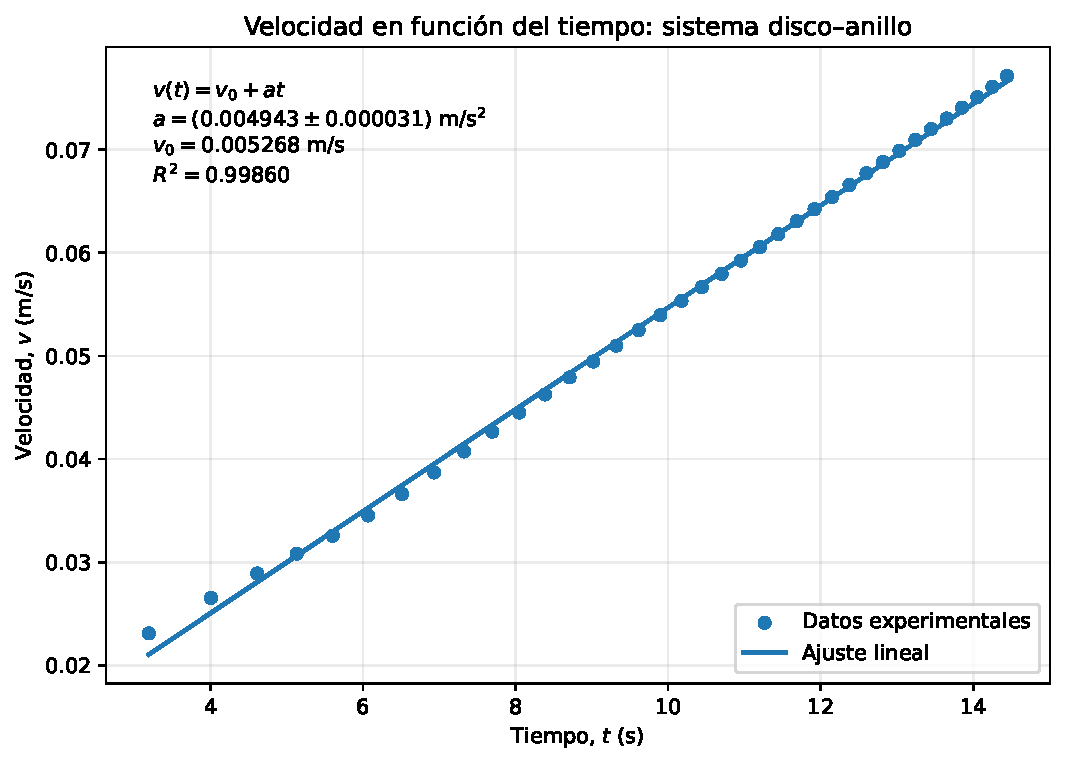
\includegraphics[width=0.82\textwidth]
    {../figuras/ajuste_velocidad.pdf}

    \vspace{0.2cm}

    \textbf{Figura 11:} Velocidad en función del tiempo y ajuste lineal
    para el sistema disco--anillo.
\end{figure}

A partir de la regresión lineal se obtuvo una aceleración

\begin{equation}
    a=(0.00494258\pm0.00003125)\,\mathrm{m/s^2}.
    \label{eq:aceleracion_experimental}
\end{equation}

Asimismo, la ordenada al origen obtenida fue

\[
    v_0=0.00526814\,\mathrm{m/s},
\]

mientras que el coeficiente de determinación del ajuste resultó

\[
    R^2=0.998603.
\]

El valor de \(R^2\), próximo a la unidad, evidencia una fuerte relación
lineal entre la velocidad y el tiempo dentro del intervalo experimental
analizado. En consecuencia, la pendiente de la recta puede emplearse como
una estimación de la aceleración lineal del sistema durante el descenso
de la masa suspendida.


% ------------------------------------------------------------
% 7.2 MOMENTO DE INERCIA EXPERIMENTAL DEL SISTEMA DISCO--ANILLO
% ------------------------------------------------------------

\subsection*{7.2. Momento de inercia experimental del sistema disco--anillo}

El momento de inercia experimental del sistema disco--anillo se determina
a partir de la expresión desarrollada en los fundamentos teóricos,

\begin{equation}
    I_{\mathrm{exp}}
    =
    \frac{m d^2(g-a)}{4a},
    \label{eq:I_experimental}
\end{equation}

donde \(m\) es la masa total suspendida, \(d\) es el diámetro del
cilindro sobre el cual se enrolla el hilo, \(g\) es la aceleración de la
gravedad y \(a\) es la aceleración obtenida mediante el ajuste lineal.

Para el presente experimento se utilizaron los valores

\[
    m=(0.2017\pm0.0001)\,\mathrm{kg},
\]

\[
    d=(0.01310\pm0.00005)\,\mathrm{m},
\]

\[
    a=(0.00494258\pm0.00003125)\,\mathrm{m/s^2},
\]

y

\[
    g=9.81\,\mathrm{m/s^2}.
\]

Sustituyendo los valores centrales en la ecuación
\eqref{eq:I_experimental},

\[
I_{D+A,\mathrm{exp}}
=
\frac{
(0.2017)(0.01310)^2
(9.81-0.00494258)
}{
4(0.00494258)
}.
\]

Por tanto,

\begin{equation}
    I_{D+A,\mathrm{exp}}
    =
    1.7167\times10^{-2}\,\mathrm{kg\,m^2}.
    \label{eq:I_exp_disco_anillo}
\end{equation}


% ------------------------------------------------------------
% 7.3 PROPAGACIÓN DE INCERTIDUMBRE DEL MOMENTO DE INERCIA
% ------------------------------------------------------------

\subsection*{7.3. Propagación de incertidumbre del momento de inercia}

Para determinar la incertidumbre asociada al momento de inercia
experimental se consideran como variables independientes las magnitudes
\(m\), \(d\) y \(a\). Para una función

\[
    I=I(m,d,a),
\]

la propagación de incertidumbres se expresa como

\[
(\delta I)^2
=
\left(
\frac{\partial I}{\partial m}\delta m
\right)^2
+
\left(
\frac{\partial I}{\partial d}\delta d
\right)^2
+
\left(
\frac{\partial I}{\partial a}\delta a
\right)^2.
\]

A partir de

\[
I=
\frac{m d^2(g-a)}{4a},
\]

las derivadas parciales correspondientes son

\[
\frac{\partial I}{\partial m}
=
\frac{d^2(g-a)}{4a},
\]

\[
\frac{\partial I}{\partial d}
=
\frac{m d(g-a)}{2a},
\]

y

\[
\frac{\partial I}{\partial a}
=
-\frac{m d^2g}{4a^2}.
\]

Por lo tanto, la incertidumbre del momento de inercia experimental queda
determinada mediante

\begin{equation}
\delta I =
\sqrt{
\left[
\frac{d^2(g-a)}{4a}\delta m
\right]^2
+
\left[
\frac{m d(g-a)}{2a}\delta d
\right]^2
+
\left[
\frac{m d^2g}{4a^2}\delta a
\right]^2
}.
\label{eq:incertidumbre_I}
\end{equation}

Sustituyendo las incertidumbres experimentales

\[
\delta m=0.0001\,\mathrm{kg},
\qquad
\delta d=0.00005\,\mathrm{m},
\]

y

\[
\delta a=0.00003125\,\mathrm{m/s^2},
\]

en la ecuación \eqref{eq:incertidumbre_I}, se obtiene

\[
\delta I_{D+A,\mathrm{exp}}
=
0.00017040\,\mathrm{kg\,m^2}.
\]

Por consiguiente, el momento de inercia experimental del sistema
disco--anillo es

\begin{equation}
I_{D+A,\mathrm{exp}}
=
(0.01716663\pm0.00017040)\,\mathrm{kg\,m^2}.
\label{eq:I_exp_final}
\end{equation}


% ------------------------------------------------------------
% 7.4 MOMENTO DE INERCIA TEÓRICO DEL DISCO
% ------------------------------------------------------------

\subsection*{7.4. Momento de inercia teórico del disco}

Para un disco homogéneo que gira alrededor de un eje perpendicular a su
plano y que pasa por su centro, el momento de inercia está dado por

\begin{equation}
I_{D,\mathrm{teo}}
=
\frac{1}{2}M_D R_D^2.
\label{eq:I_disco_teorico}
\end{equation}

Utilizando

\[
M_D=(1.4544\pm0.0001)\,\mathrm{kg},
\]

y

\[
R_D=(0.11430\pm0.00050)\,\mathrm{m},
\]

se obtiene

\[
I_{D,\mathrm{teo}}
=
\frac{1}{2}(1.4544)(0.11430)^2,
\]

de donde

\[
I_{D,\mathrm{teo}}
=
0.00950050\,\mathrm{kg\,m^2}.
\]

La incertidumbre asociada se determinó mediante

\[
\delta I_D=
\sqrt{
\left(
\frac{R_D^2}{2}\delta M_D
\right)^2
+
\left(
M_D R_D\delta R_D
\right)^2
},
\]

obteniéndose finalmente

\begin{equation}
I_{D,\mathrm{teo}}
=
(0.00950050\pm0.00008312)\,\mathrm{kg\,m^2}.
\label{eq:I_disco_teorico_final}
\end{equation}


% ------------------------------------------------------------
% 7.5 MOMENTO DE INERCIA TEÓRICO DEL ANILLO
% ------------------------------------------------------------

\subsection*{7.5. Momento de inercia teórico del anillo}

Para el anillo, el momento de inercia teórico respecto de su eje central
se determina mediante

\begin{equation}
I_{A,\mathrm{teo}}
=
\frac{1}{2}M_A
\left(
R_i^2+R_e^2
\right).
\label{eq:I_anillo_teorico}
\end{equation}

Considerando

\[
M_A=(1.4466\pm0.0001)\,\mathrm{kg},
\]

\[
R_i=(0.053575\pm0.000050)\,\mathrm{m},
\]

y

\[
R_e=(0.063825\pm0.000050)\,\mathrm{m},
\]

se obtiene

\[
I_{A,\mathrm{teo}}
=
\frac{1}{2}(1.4466)
\left[
(0.053575)^2+(0.063825)^2
\right],
\]

por lo que

\[
I_{A,\mathrm{teo}}
=
0.00502253\,\mathrm{kg\,m^2}.
\]

La incertidumbre correspondiente se calculó mediante

\[
\delta I_A=
\sqrt{
\left[
\frac{R_i^2+R_e^2}{2}\delta M_A
\right]^2
+
\left(
M_A R_i\delta R_i
\right)^2
+
\left(
M_A R_e\delta R_e
\right)^2
}.
\]

De esta manera,

\begin{equation}
I_{A,\mathrm{teo}}
=
(0.00502253\pm0.00000604)\,\mathrm{kg\,m^2}.
\label{eq:I_anillo_teorico_final}
\end{equation}


% ------------------------------------------------------------
% 7.6 MOMENTO DE INERCIA TEÓRICO DEL SISTEMA
% ------------------------------------------------------------

\subsection*{7.6. Momento de inercia teórico del sistema disco--anillo}

Al encontrarse el disco y el anillo rotando alrededor del mismo eje, el
momento de inercia teórico total se obtiene mediante la suma de sus
momentos de inercia individuales:

\[
I_{D+A,\mathrm{teo}}
=
I_{D,\mathrm{teo}}
+
I_{A,\mathrm{teo}}.
\]

Por tanto,

\[
I_{D+A,\mathrm{teo}}
=
0.00950050
+
0.00502253,
\]

y se obtiene

\[
I_{D+A,\mathrm{teo}}
=
0.01452303\,\mathrm{kg\,m^2}.
\]

Considerando independientes las incertidumbres del disco y del anillo,

\[
\delta I_{D+A,\mathrm{teo}}
=
\sqrt{
(\delta I_D)^2+
(\delta I_A)^2
},
\]

de donde

\[
\delta I_{D+A,\mathrm{teo}}
=
0.00008334\,\mathrm{kg\,m^2}.
\]

Así, el resultado teórico total es

\begin{equation}
I_{D+A,\mathrm{teo}}
=
(0.01452303\pm0.00008334)\,\mathrm{kg\,m^2}.
\label{eq:I_teorico_total}
\end{equation}


% ------------------------------------------------------------
% 7.7 COMPARACIÓN ENTRE LOS RESULTADOS
% ------------------------------------------------------------

\subsection*{7.7. Comparación entre los resultados experimental y teórico}

Para cuantificar la diferencia entre el resultado experimental y el
valor teórico se calculó la discrepancia porcentual mediante

\begin{equation}
\text{Discrepancia}=
\frac{
\left|
I_{D+A,\mathrm{exp}}-I_{D+A,\mathrm{teo}}
\right|
}{
I_{D+A,\mathrm{teo}}
}
\times100\%.
\label{eq:discrepancia}
\end{equation}

Sustituyendo los resultados obtenidos,

\[
\text{Discrepancia}
=
\frac{
|0.01716663-0.01452303|
}{
0.01452303
}
\times100\%,
\]

se obtiene

\begin{equation}
\boxed{
\text{Discrepancia}=18.20\%
}
\end{equation}

Adicionalmente, se evaluó la diferencia entre ambos resultados respecto
de su incertidumbre combinada mediante

\[
z=
\frac{
\left|
I_{D+A,\mathrm{exp}}-I_{D+A,\mathrm{teo}}
\right|
}{
\sqrt{
(\delta I_{D+A,\mathrm{exp}})^2+
(\delta I_{D+A,\mathrm{teo}})^2
}
}.
\]

El valor obtenido fue

\[
z=13.94.
\]

Este resultado indica que la diferencia entre los valores experimental
y teórico es considerablemente mayor que la incertidumbre combinada
estimada a partir de las magnitudes medidas. Por ello, la discrepancia
observada no puede atribuirse únicamente a las incertidumbres aleatorias
consideradas en la propagación, sino que sugiere la presencia de efectos
sistemáticos no incluidos en el modelo ideal.


% ------------------------------------------------------------
% CUADRO RESUMEN
% ------------------------------------------------------------

\subsection*{7.8. Resumen de resultados}

Los principales resultados obtenidos durante el análisis se presentan
en el Cuadro 5.

\begin{table}[h!]
\centering
\renewcommand{\arraystretch}{1.35}

\begin{tabular}{lc}
\hline
\textbf{Magnitud} & \textbf{Resultado} \\
\hline

Aceleración experimental
&
\((0.00494258\pm0.00003125)\,\mathrm{m/s^2}\)
\\

Momento de inercia experimental disco--anillo
&
\((0.01716663\pm0.00017040)\,\mathrm{kg\,m^2}\)
\\

Momento de inercia teórico del disco
&
\((0.00950050\pm0.00008312)\,\mathrm{kg\,m^2}\)
\\

Momento de inercia teórico del anillo
&
\((0.00502253\pm0.00000604)\,\mathrm{kg\,m^2}\)
\\

Momento de inercia teórico disco--anillo
&
\((0.01452303\pm0.00008334)\,\mathrm{kg\,m^2}\)
\\

Discrepancia porcentual
&
\(18.20\%\)
\\

Discrepancia normalizada
&
\(z=13.94\)
\\

\hline
\end{tabular}

\vspace{0.2cm}

\textbf{Cuadro 5:} Resumen de los resultados obtenidos para el sistema
disco--anillo.

\end{table}

% ============================================================
% 8. DISCUSIÓN DE RESULTADOS
% ============================================================

\newpage
\section*{8. DISCUSIÓN DE RESULTADOS}
\addcontentsline{toc}{section}{8. DISCUSIÓN DE RESULTADOS}
\sectionline

Los datos de velocidad en función del tiempo presentaron un
comportamiento aproximadamente lineal. El ajuste realizado mediante
Python proporcionó un coeficiente de determinación

\[
R^2=0.998603,
\]

lo que indica que el modelo lineal describe adecuadamente la evolución
de la velocidad durante el intervalo analizado. La aceleración obtenida
a partir de la pendiente fue

\[
a=(0.00494258\pm0.00003125)\,\mathrm{m/s^2}.
\]

El elevado valor de \(R^2\) muestra que la dispersión de los datos
respecto de la recta de ajuste es pequeña. Sin embargo, una buena
linealidad no implica necesariamente que el sistema experimental
reproduzca de manera exacta el modelo dinámico ideal, ya que pueden
existir efectos sistemáticos que modifiquen la aceleración manteniendo
un comportamiento aproximadamente lineal.

A partir de la aceleración experimental y de los parámetros del sistema
se obtuvo para el conjunto disco--anillo

\[
I_{D+A,\mathrm{exp}}
=
(0.01716663\pm0.00017040)\,\mathrm{kg\,m^2}.
\]

Por otro lado, empleando las masas y dimensiones geométricas medidas, se
obtuvieron los momentos de inercia teóricos

\[
I_{D,\mathrm{teo}}
=
(0.00950050\pm0.00008312)\,\mathrm{kg\,m^2},
\]

para el disco, y

\[
I_{A,\mathrm{teo}}
=
(0.00502253\pm0.00000604)\,\mathrm{kg\,m^2},
\]

para el anillo. La suma de ambas contribuciones proporcionó

\[
I_{D+A,\mathrm{teo}}
=
(0.01452303\pm0.00008334)\,\mathrm{kg\,m^2}.
\]

El momento de inercia determinado experimentalmente resultó mayor que
el valor calculado teóricamente. La diferencia absoluta entre ambos
resultados fue

\[
\left|
I_{D+A,\mathrm{exp}}-I_{D+A,\mathrm{teo}}
\right|
=
0.00264360\,\mathrm{kg\,m^2},
\]

correspondiente a una discrepancia porcentual de

\[
18.20\%.
\]

Asimismo, la discrepancia normalizada obtenida fue \(z=13.94\). Este
valor indica que la separación entre los resultados experimental y
teórico es considerablemente mayor que la incertidumbre combinada
estimada a partir de las magnitudes medidas. En consecuencia, la
diferencia observada no puede explicarse únicamente mediante las
incertidumbres aleatorias consideradas en la propagación.

Una de las principales causas posibles de esta discrepancia es la
presencia de fricción en el eje de rotación y en la polea. En la
deducción de la expresión empleada para calcular el momento de inercia
experimental se considera que el torque producido por la tensión del
hilo es utilizado íntegramente para acelerar el sistema. En el montaje
real, parte de este torque debe compensar los efectos de rozamiento. Si
estos efectos no se incorporan explícitamente al modelo, la aceleración
observada puede ser menor que la predicha para un sistema ideal. Debido
a que la aceleración aparece en el denominador de la expresión utilizada
para determinar \(I_{\mathrm{exp}}\), una disminución de la aceleración
conduce a una sobreestimación del momento de inercia, consistente con el
resultado obtenido experimentalmente.

También pueden contribuir a la discrepancia las características del
sistema hilo--polea. El modelo supone un hilo ideal, de masa despreciable
e inextensible, sin deslizamiento sobre el cilindro. En la práctica,
pequeñas deformaciones, deslizamientos o variaciones en el radio efectivo
de enrollamiento modifican la relación entre la aceleración lineal y la
aceleración angular. Además, la polea posee un momento de inercia propio,
el cual no fue incluido explícitamente en el modelo utilizado.

Otro factor particularmente sensible es la medición del diámetro del
cilindro sobre el cual se enrolla el hilo. De acuerdo con la expresión

\[
I_{\mathrm{exp}}
=
\frac{m d^2(g-a)}{4a},
\]

el momento de inercia depende cuadráticamente de \(d\). Por esta razón,
una desviación en la determinación del diámetro efectivo produce una
variación apreciable en el momento de inercia calculado. De forma
similar, la determinación de la aceleración constituye una variable
crítica debido a su presencia en el denominador de la expresión.

Las incertidumbres calculadas representan principalmente la contribución
de las magnitudes medidas y de la regresión lineal. Sin embargo, no
incorporan necesariamente todos los efectos sistemáticos presentes en
el montaje, como la fricción, el momento de inercia de la polea, posibles
desalineamientos, el comportamiento no ideal del hilo o variaciones del
radio efectivo durante su desenrollamiento. Esto permite explicar por
qué se obtuvo un ajuste lineal con \(R^2\) elevado y, simultáneamente,
una diferencia significativa entre los momentos de inercia experimental
y teórico.

Finalmente, debido a que se dispuso de una única serie completa de datos
dinámicos para el sistema disco--anillo, la comparación experimental se
realizó para el conjunto completo. Los momentos de inercia individuales
del disco y del anillo fueron determinados teóricamente a partir de sus
respectivas masas y dimensiones geométricas. Por este motivo, no se
reportan valores experimentales independientes para cada componente,
evitando inferir resultados que no se encuentran respaldados por los
datos registrados.

% ============================================================
% 9. CONCLUSIONES
% ============================================================

\newpage
\section*{9. CONCLUSIONES}
\addcontentsline{toc}{section}{9. CONCLUSIONES}
\sectionline

\begin{enumerate}

    \item Se determinó la aceleración lineal del sistema disco--anillo
    mediante un ajuste lineal de 37 datos experimentales de velocidad
    en función del tiempo. El resultado obtenido fue

    \[
    a=(0.00494258\pm0.00003125)\,\mathrm{m/s^2},
    \]

    con un coeficiente de determinación \(R^2=0.998603\), evidenciando
    una elevada linealidad de los datos experimentales.

    \item A partir de la dinámica traslacional y rotacional del sistema
    se obtuvo un momento de inercia experimental

    \[
    I_{D+A,\mathrm{exp}}
    =
    (0.01716663\pm0.00017040)\,\mathrm{kg\,m^2}.
    \]

    \item Mediante las masas y dimensiones geométricas medidas se
    obtuvieron los momentos de inercia teóricos del disco y del anillo,

    \[
    I_{D,\mathrm{teo}}
    =
    (0.00950050\pm0.00008312)\,\mathrm{kg\,m^2},
    \]

    y

    \[
    I_{A,\mathrm{teo}}
    =
    (0.00502253\pm0.00000604)\,\mathrm{kg\,m^2},
    \]

    respectivamente. La suma de ambas contribuciones produjo

    \[
    I_{D+A,\mathrm{teo}}
    =
    (0.01452303\pm0.00008334)\,\mathrm{kg\,m^2}.
    \]

    \item La comparación entre los resultados experimental y teórico
    produjo una discrepancia porcentual de \(18.20\%\). Además, se
    obtuvo una discrepancia normalizada \(z=13.94\), lo cual indica que
    la diferencia observada supera ampliamente la incertidumbre
    combinada estimada.

    \item La sobreestimación del momento de inercia experimental es
    compatible con la presencia de efectos sistemáticos no considerados
    en el modelo ideal, entre ellos la fricción en el eje y la polea,
    el momento de inercia propio de esta última, las características
    no ideales del hilo y posibles variaciones en el radio efectivo de
    enrollamiento.

    \item La experiencia permitió verificar experimentalmente la
    relación entre el movimiento traslacional de una masa suspendida y
    la dinámica rotacional del sistema. No obstante, para determinar
    experimentalmente por separado los momentos de inercia del disco y
    del anillo sería necesario disponer de una segunda serie de datos
    correspondiente al movimiento del disco sin el anillo.

\end{enumerate}


% ============================================================
% 10. BIBLIOGRAFÍA
% ============================================================

\newpage
\section*{10. BIBLIOGRAFÍA}
\addcontentsline{toc}{section}{10. BIBLIOGRAFÍA}
\sectionline

\begin{thebibliography}{99}

\bibitem{alonso_finn}
Alonso, M. y Finn, E. J.
\textit{Física: Curso completo, Vol. I}.
Addison-Wesley Iberoamericana, 1995.

\bibitem{giancoli}
Giancoli, D. C.
\textit{Física: Principios con aplicaciones}.
6.a ed., Pearson Educación, 2006.

\bibitem{halliday}
Halliday, D., Resnick, R. y Walker, J.
\textit{Fundamentos de física}.
8.a ed., Grupo Editorial Patria, 2009.

\bibitem{serway}
Serway, R. A. y Jewett, J. W.
\textit{Física para ciencias e ingeniería, Vol. 1}.
7.a ed., Cengage Learning, 2009.

\bibitem{sears}
Sears, F. W., Zemansky, M. W. y Young, H. D.
\textit{Física universitaria}.
11.a ed., Pearson Educación, 2004.

\bibitem{tipler}
Tipler, P. A. y Mosca, G.
\textit{Física para la ciencia y la tecnología, Vol. 1}.
6.a ed., Editorial Reverté, 2008.

\end{thebibliography}

% ============================================================
% 11. ANEXOS
% ============================================================

\newpage
\section*{11. ANEXOS}
\addcontentsline{toc}{section}{11. ANEXOS}
\sectionline

\subsection*{11.1. Repositorio del laboratorio}

Los archivos utilizados para el procesamiento de datos, elaboración de
gráficas y desarrollo del informe se encuentran disponibles en el
repositorio de GitHub del laboratorio:

\begin{center}
\url{https://github.com/alexandradeOz-wq/FISICA-2-LABORATORY}
\end{center}

El repositorio contiene los códigos desarrollados en Python para el
ajuste de los datos experimentales y el cálculo de los momentos de
inercia, así como el código fuente en \LaTeX{} empleado para la
elaboración del presente informe.


\subsection*{11.2. Participación de los integrantes}

\begin{table}[h!]
\centering
\renewcommand{\arraystretch}{1.3}
\begin{tabular}{p{0.28\textwidth} p{0.62\textwidth}}
\hline
\textbf{Integrante} & \textbf{Participación} \\
\hline

Moreno Cabanillas, Alexandra Romina &
Toma y organización de datos experimentales, procesamiento de datos
mediante Python, elaboración de gráficas y redacción del informe en
\LaTeX{}. \\

Macuri Torres, Alessandro Omar &
Montaje y ejecución del experimento, medición de las magnitudes físicas,
verificación de cálculos y participación en el análisis y discusión de
los resultados. \\

\hline
\end{tabular}

\vspace{0.2cm}
\textbf{Cuadro 6:} Participación de los integrantes en el desarrollo
del laboratorio.
\end{table}

\end{document}